\documentclass[11pt]{article}

    \usepackage[breakable]{tcolorbox}
    \usepackage{parskip} % Stop auto-indenting (to mimic markdown behaviour)
    

    % Basic figure setup, for now with no caption control since it's done
    % automatically by Pandoc (which extracts ![](path) syntax from Markdown).
    \usepackage{graphicx}
    % Keep aspect ratio if custom image width or height is specified
    \setkeys{Gin}{keepaspectratio}
    % Maintain compatibility with old templates. Remove in nbconvert 6.0
    \let\Oldincludegraphics\includegraphics
    % Ensure that by default, figures have no caption (until we provide a
    % proper Figure object with a Caption API and a way to capture that
    % in the conversion process - todo).
    \usepackage{caption}
    \DeclareCaptionFormat{nocaption}{}
    \captionsetup{format=nocaption,aboveskip=0pt,belowskip=0pt}

    \usepackage{float}
    \floatplacement{figure}{H} % forces figures to be placed at the correct location
    \usepackage{xcolor} % Allow colors to be defined
    \usepackage{enumerate} % Needed for markdown enumerations to work
    \usepackage{geometry} % Used to adjust the document margins
    \usepackage{amsmath} % Equations
    \usepackage{amssymb} % Equations
    \usepackage{textcomp} % defines textquotesingle
    % Hack from http://tex.stackexchange.com/a/47451/13684:
    \AtBeginDocument{%
        \def\PYZsq{\textquotesingle}% Upright quotes in Pygmentized code
    }
    \usepackage{upquote} % Upright quotes for verbatim code
    \usepackage{eurosym} % defines \euro

    \usepackage{iftex}
    \ifPDFTeX
        \usepackage[T1]{fontenc}
        \usepackage[utf8]{inputenc}
    \else
        \usepackage{fontspec}
        \usepackage{unicode-math}
    \fi

    \usepackage{fancyvrb} % verbatim replacement that allows latex
    \usepackage{grffile} % extends the file name processing of package graphics
                         % to support a larger range
    \makeatletter % fix for old versions of grffile with XeLaTeX
    \@ifpackagelater{grffile}{2019/11/01}
    {
      % Do nothing on new versions
    }
    {
      \def\Gread@@xetex#1{%
        \IfFileExists{"\Gin@base".bb}%
        {\Gread@eps{\Gin@base.bb}}%
        {\Gread@@xetex@aux#1}%
      }
    }
    \makeatother
    \usepackage[Export]{adjustbox} % Used to constrain images to a maximum size
    \adjustboxset{max size={0.9\linewidth}{0.9\paperheight}}

    % The hyperref package gives us a pdf with properly built
    % internal navigation ('pdf bookmarks' for the table of contents,
    % internal cross-reference links, web links for URLs, etc.)
    \usepackage{hyperref}
    % The default LaTeX title has an obnoxious amount of whitespace. By default,
    % titling removes some of it. It also provides customization options.
    \usepackage{titling}
    \usepackage{longtable} % longtable support required by pandoc >1.10
    \usepackage{booktabs}  % table support for pandoc > 1.12.2
    \usepackage{array}     % table support for pandoc >= 2.11.3
    \usepackage{calc}      % table minipage width calculation for pandoc >= 2.11.1
    \usepackage[inline]{enumitem} % IRkernel/repr support (it uses the enumerate* environment)
    \usepackage[normalem]{ulem} % ulem is needed to support strikethroughs (\sout)
                                % normalem makes italics be italics, not underlines
    \usepackage{soul}      % strikethrough (\st) support for pandoc >= 3.0.0
    \usepackage{mathrsfs}
    

    
    % Colors for the hyperref package
    \definecolor{urlcolor}{rgb}{0,.145,.698}
    \definecolor{linkcolor}{rgb}{.71,0.21,0.01}
    \definecolor{citecolor}{rgb}{.12,.54,.11}

    % ANSI colors
    \definecolor{ansi-black}{HTML}{3E424D}
    \definecolor{ansi-black-intense}{HTML}{282C36}
    \definecolor{ansi-red}{HTML}{E75C58}
    \definecolor{ansi-red-intense}{HTML}{B22B31}
    \definecolor{ansi-green}{HTML}{00A250}
    \definecolor{ansi-green-intense}{HTML}{007427}
    \definecolor{ansi-yellow}{HTML}{DDB62B}
    \definecolor{ansi-yellow-intense}{HTML}{B27D12}
    \definecolor{ansi-blue}{HTML}{208FFB}
    \definecolor{ansi-blue-intense}{HTML}{0065CA}
    \definecolor{ansi-magenta}{HTML}{D160C4}
    \definecolor{ansi-magenta-intense}{HTML}{A03196}
    \definecolor{ansi-cyan}{HTML}{60C6C8}
    \definecolor{ansi-cyan-intense}{HTML}{258F8F}
    \definecolor{ansi-white}{HTML}{C5C1B4}
    \definecolor{ansi-white-intense}{HTML}{A1A6B2}
    \definecolor{ansi-default-inverse-fg}{HTML}{FFFFFF}
    \definecolor{ansi-default-inverse-bg}{HTML}{000000}

    % common color for the border for error outputs.
    \definecolor{outerrorbackground}{HTML}{FFDFDF}

    % commands and environments needed by pandoc snippets
    % extracted from the output of `pandoc -s`
    \providecommand{\tightlist}{%
      \setlength{\itemsep}{0pt}\setlength{\parskip}{0pt}}
    \DefineVerbatimEnvironment{Highlighting}{Verbatim}{commandchars=\\\{\}}
    % Add ',fontsize=\small' for more characters per line
    \newenvironment{Shaded}{}{}
    \newcommand{\KeywordTok}[1]{\textcolor[rgb]{0.00,0.44,0.13}{\textbf{{#1}}}}
    \newcommand{\DataTypeTok}[1]{\textcolor[rgb]{0.56,0.13,0.00}{{#1}}}
    \newcommand{\DecValTok}[1]{\textcolor[rgb]{0.25,0.63,0.44}{{#1}}}
    \newcommand{\BaseNTok}[1]{\textcolor[rgb]{0.25,0.63,0.44}{{#1}}}
    \newcommand{\FloatTok}[1]{\textcolor[rgb]{0.25,0.63,0.44}{{#1}}}
    \newcommand{\CharTok}[1]{\textcolor[rgb]{0.25,0.44,0.63}{{#1}}}
    \newcommand{\StringTok}[1]{\textcolor[rgb]{0.25,0.44,0.63}{{#1}}}
    \newcommand{\CommentTok}[1]{\textcolor[rgb]{0.38,0.63,0.69}{\textit{{#1}}}}
    \newcommand{\OtherTok}[1]{\textcolor[rgb]{0.00,0.44,0.13}{{#1}}}
    \newcommand{\AlertTok}[1]{\textcolor[rgb]{1.00,0.00,0.00}{\textbf{{#1}}}}
    \newcommand{\FunctionTok}[1]{\textcolor[rgb]{0.02,0.16,0.49}{{#1}}}
    \newcommand{\RegionMarkerTok}[1]{{#1}}
    \newcommand{\ErrorTok}[1]{\textcolor[rgb]{1.00,0.00,0.00}{\textbf{{#1}}}}
    \newcommand{\NormalTok}[1]{{#1}}

    % Additional commands for more recent versions of Pandoc
    \newcommand{\ConstantTok}[1]{\textcolor[rgb]{0.53,0.00,0.00}{{#1}}}
    \newcommand{\SpecialCharTok}[1]{\textcolor[rgb]{0.25,0.44,0.63}{{#1}}}
    \newcommand{\VerbatimStringTok}[1]{\textcolor[rgb]{0.25,0.44,0.63}{{#1}}}
    \newcommand{\SpecialStringTok}[1]{\textcolor[rgb]{0.73,0.40,0.53}{{#1}}}
    \newcommand{\ImportTok}[1]{{#1}}
    \newcommand{\DocumentationTok}[1]{\textcolor[rgb]{0.73,0.13,0.13}{\textit{{#1}}}}
    \newcommand{\AnnotationTok}[1]{\textcolor[rgb]{0.38,0.63,0.69}{\textbf{\textit{{#1}}}}}
    \newcommand{\CommentVarTok}[1]{\textcolor[rgb]{0.38,0.63,0.69}{\textbf{\textit{{#1}}}}}
    \newcommand{\VariableTok}[1]{\textcolor[rgb]{0.10,0.09,0.49}{{#1}}}
    \newcommand{\ControlFlowTok}[1]{\textcolor[rgb]{0.00,0.44,0.13}{\textbf{{#1}}}}
    \newcommand{\OperatorTok}[1]{\textcolor[rgb]{0.40,0.40,0.40}{{#1}}}
    \newcommand{\BuiltInTok}[1]{{#1}}
    \newcommand{\ExtensionTok}[1]{{#1}}
    \newcommand{\PreprocessorTok}[1]{\textcolor[rgb]{0.74,0.48,0.00}{{#1}}}
    \newcommand{\AttributeTok}[1]{\textcolor[rgb]{0.49,0.56,0.16}{{#1}}}
    \newcommand{\InformationTok}[1]{\textcolor[rgb]{0.38,0.63,0.69}{\textbf{\textit{{#1}}}}}
    \newcommand{\WarningTok}[1]{\textcolor[rgb]{0.38,0.63,0.69}{\textbf{\textit{{#1}}}}}
    \makeatletter
    \newsavebox\pandoc@box
    \newcommand*\pandocbounded[1]{%
      \sbox\pandoc@box{#1}%
      % scaling factors for width and height
      \Gscale@div\@tempa\textheight{\dimexpr\ht\pandoc@box+\dp\pandoc@box\relax}%
      \Gscale@div\@tempb\linewidth{\wd\pandoc@box}%
      % select the smaller of both
      \ifdim\@tempb\p@<\@tempa\p@
        \let\@tempa\@tempb
      \fi
      % scaling accordingly (\@tempa < 1)
      \ifdim\@tempa\p@<\p@
        \scalebox{\@tempa}{\usebox\pandoc@box}%
      % scaling not needed, use as it is
      \else
        \usebox{\pandoc@box}%
      \fi
    }
    \makeatother

    % Define a nice break command that doesn't care if a line doesn't already
    % exist.
    \def\br{\hspace*{\fill} \\* }
    % Math Jax compatibility definitions
    \def\gt{>}
    \def\lt{<}
    \let\Oldtex\TeX
    \let\Oldlatex\LaTeX
    \renewcommand{\TeX}{\textrm{\Oldtex}}
    \renewcommand{\LaTeX}{\textrm{\Oldlatex}}
    % Document parameters
    % Document title
    \title{The Charge Solver in tidy3d}
    \author{Roman Panshin}
    \date{13 August 2026}

    
    
    
    
    
    
% Pygments definitions
\makeatletter
\def\PY@reset{\let\PY@it=\relax \let\PY@bf=\relax%
    \let\PY@ul=\relax \let\PY@tc=\relax%
    \let\PY@bc=\relax \let\PY@ff=\relax}
\def\PY@tok#1{\csname PY@tok@#1\endcsname}
\def\PY@toks#1+{\ifx\relax#1\empty\else%
    \PY@tok{#1}\expandafter\PY@toks\fi}
\def\PY@do#1{\PY@bc{\PY@tc{\PY@ul{%
    \PY@it{\PY@bf{\PY@ff{#1}}}}}}}
\def\PY#1#2{\PY@reset\PY@toks#1+\relax+\PY@do{#2}}

\@namedef{PY@tok@w}{\def\PY@tc##1{\textcolor[rgb]{0.73,0.73,0.73}{##1}}}
\@namedef{PY@tok@c}{\let\PY@it=\textit\def\PY@tc##1{\textcolor[rgb]{0.24,0.48,0.48}{##1}}}
\@namedef{PY@tok@cp}{\def\PY@tc##1{\textcolor[rgb]{0.61,0.40,0.00}{##1}}}
\@namedef{PY@tok@k}{\let\PY@bf=\textbf\def\PY@tc##1{\textcolor[rgb]{0.00,0.50,0.00}{##1}}}
\@namedef{PY@tok@kp}{\def\PY@tc##1{\textcolor[rgb]{0.00,0.50,0.00}{##1}}}
\@namedef{PY@tok@kt}{\def\PY@tc##1{\textcolor[rgb]{0.69,0.00,0.25}{##1}}}
\@namedef{PY@tok@o}{\def\PY@tc##1{\textcolor[rgb]{0.40,0.40,0.40}{##1}}}
\@namedef{PY@tok@ow}{\let\PY@bf=\textbf\def\PY@tc##1{\textcolor[rgb]{0.67,0.13,1.00}{##1}}}
\@namedef{PY@tok@nb}{\def\PY@tc##1{\textcolor[rgb]{0.00,0.50,0.00}{##1}}}
\@namedef{PY@tok@nf}{\def\PY@tc##1{\textcolor[rgb]{0.00,0.00,1.00}{##1}}}
\@namedef{PY@tok@nc}{\let\PY@bf=\textbf\def\PY@tc##1{\textcolor[rgb]{0.00,0.00,1.00}{##1}}}
\@namedef{PY@tok@nn}{\let\PY@bf=\textbf\def\PY@tc##1{\textcolor[rgb]{0.00,0.00,1.00}{##1}}}
\@namedef{PY@tok@ne}{\let\PY@bf=\textbf\def\PY@tc##1{\textcolor[rgb]{0.80,0.25,0.22}{##1}}}
\@namedef{PY@tok@nv}{\def\PY@tc##1{\textcolor[rgb]{0.10,0.09,0.49}{##1}}}
\@namedef{PY@tok@no}{\def\PY@tc##1{\textcolor[rgb]{0.53,0.00,0.00}{##1}}}
\@namedef{PY@tok@nl}{\def\PY@tc##1{\textcolor[rgb]{0.46,0.46,0.00}{##1}}}
\@namedef{PY@tok@ni}{\let\PY@bf=\textbf\def\PY@tc##1{\textcolor[rgb]{0.44,0.44,0.44}{##1}}}
\@namedef{PY@tok@na}{\def\PY@tc##1{\textcolor[rgb]{0.41,0.47,0.13}{##1}}}
\@namedef{PY@tok@nt}{\let\PY@bf=\textbf\def\PY@tc##1{\textcolor[rgb]{0.00,0.50,0.00}{##1}}}
\@namedef{PY@tok@nd}{\def\PY@tc##1{\textcolor[rgb]{0.67,0.13,1.00}{##1}}}
\@namedef{PY@tok@s}{\def\PY@tc##1{\textcolor[rgb]{0.73,0.13,0.13}{##1}}}
\@namedef{PY@tok@sd}{\let\PY@it=\textit\def\PY@tc##1{\textcolor[rgb]{0.73,0.13,0.13}{##1}}}
\@namedef{PY@tok@si}{\let\PY@bf=\textbf\def\PY@tc##1{\textcolor[rgb]{0.64,0.35,0.47}{##1}}}
\@namedef{PY@tok@se}{\let\PY@bf=\textbf\def\PY@tc##1{\textcolor[rgb]{0.67,0.36,0.12}{##1}}}
\@namedef{PY@tok@sr}{\def\PY@tc##1{\textcolor[rgb]{0.64,0.35,0.47}{##1}}}
\@namedef{PY@tok@ss}{\def\PY@tc##1{\textcolor[rgb]{0.10,0.09,0.49}{##1}}}
\@namedef{PY@tok@sx}{\def\PY@tc##1{\textcolor[rgb]{0.00,0.50,0.00}{##1}}}
\@namedef{PY@tok@m}{\def\PY@tc##1{\textcolor[rgb]{0.40,0.40,0.40}{##1}}}
\@namedef{PY@tok@gh}{\let\PY@bf=\textbf\def\PY@tc##1{\textcolor[rgb]{0.00,0.00,0.50}{##1}}}
\@namedef{PY@tok@gu}{\let\PY@bf=\textbf\def\PY@tc##1{\textcolor[rgb]{0.50,0.00,0.50}{##1}}}
\@namedef{PY@tok@gd}{\def\PY@tc##1{\textcolor[rgb]{0.63,0.00,0.00}{##1}}}
\@namedef{PY@tok@gi}{\def\PY@tc##1{\textcolor[rgb]{0.00,0.52,0.00}{##1}}}
\@namedef{PY@tok@gr}{\def\PY@tc##1{\textcolor[rgb]{0.89,0.00,0.00}{##1}}}
\@namedef{PY@tok@ge}{\let\PY@it=\textit}
\@namedef{PY@tok@gs}{\let\PY@bf=\textbf}
\@namedef{PY@tok@ges}{\let\PY@bf=\textbf\let\PY@it=\textit}
\@namedef{PY@tok@gp}{\let\PY@bf=\textbf\def\PY@tc##1{\textcolor[rgb]{0.00,0.00,0.50}{##1}}}
\@namedef{PY@tok@go}{\def\PY@tc##1{\textcolor[rgb]{0.44,0.44,0.44}{##1}}}
\@namedef{PY@tok@gt}{\def\PY@tc##1{\textcolor[rgb]{0.00,0.27,0.87}{##1}}}
\@namedef{PY@tok@err}{\def\PY@bc##1{{\setlength{\fboxsep}{\string -\fboxrule}\fcolorbox[rgb]{1.00,0.00,0.00}{1,1,1}{\strut ##1}}}}
\@namedef{PY@tok@kc}{\let\PY@bf=\textbf\def\PY@tc##1{\textcolor[rgb]{0.00,0.50,0.00}{##1}}}
\@namedef{PY@tok@kd}{\let\PY@bf=\textbf\def\PY@tc##1{\textcolor[rgb]{0.00,0.50,0.00}{##1}}}
\@namedef{PY@tok@kn}{\let\PY@bf=\textbf\def\PY@tc##1{\textcolor[rgb]{0.00,0.50,0.00}{##1}}}
\@namedef{PY@tok@kr}{\let\PY@bf=\textbf\def\PY@tc##1{\textcolor[rgb]{0.00,0.50,0.00}{##1}}}
\@namedef{PY@tok@bp}{\def\PY@tc##1{\textcolor[rgb]{0.00,0.50,0.00}{##1}}}
\@namedef{PY@tok@fm}{\def\PY@tc##1{\textcolor[rgb]{0.00,0.00,1.00}{##1}}}
\@namedef{PY@tok@vc}{\def\PY@tc##1{\textcolor[rgb]{0.10,0.09,0.49}{##1}}}
\@namedef{PY@tok@vg}{\def\PY@tc##1{\textcolor[rgb]{0.10,0.09,0.49}{##1}}}
\@namedef{PY@tok@vi}{\def\PY@tc##1{\textcolor[rgb]{0.10,0.09,0.49}{##1}}}
\@namedef{PY@tok@vm}{\def\PY@tc##1{\textcolor[rgb]{0.10,0.09,0.49}{##1}}}
\@namedef{PY@tok@sa}{\def\PY@tc##1{\textcolor[rgb]{0.73,0.13,0.13}{##1}}}
\@namedef{PY@tok@sb}{\def\PY@tc##1{\textcolor[rgb]{0.73,0.13,0.13}{##1}}}
\@namedef{PY@tok@sc}{\def\PY@tc##1{\textcolor[rgb]{0.73,0.13,0.13}{##1}}}
\@namedef{PY@tok@dl}{\def\PY@tc##1{\textcolor[rgb]{0.73,0.13,0.13}{##1}}}
\@namedef{PY@tok@s2}{\def\PY@tc##1{\textcolor[rgb]{0.73,0.13,0.13}{##1}}}
\@namedef{PY@tok@sh}{\def\PY@tc##1{\textcolor[rgb]{0.73,0.13,0.13}{##1}}}
\@namedef{PY@tok@s1}{\def\PY@tc##1{\textcolor[rgb]{0.73,0.13,0.13}{##1}}}
\@namedef{PY@tok@mb}{\def\PY@tc##1{\textcolor[rgb]{0.40,0.40,0.40}{##1}}}
\@namedef{PY@tok@mf}{\def\PY@tc##1{\textcolor[rgb]{0.40,0.40,0.40}{##1}}}
\@namedef{PY@tok@mh}{\def\PY@tc##1{\textcolor[rgb]{0.40,0.40,0.40}{##1}}}
\@namedef{PY@tok@mi}{\def\PY@tc##1{\textcolor[rgb]{0.40,0.40,0.40}{##1}}}
\@namedef{PY@tok@il}{\def\PY@tc##1{\textcolor[rgb]{0.40,0.40,0.40}{##1}}}
\@namedef{PY@tok@mo}{\def\PY@tc##1{\textcolor[rgb]{0.40,0.40,0.40}{##1}}}
\@namedef{PY@tok@ch}{\let\PY@it=\textit\def\PY@tc##1{\textcolor[rgb]{0.24,0.48,0.48}{##1}}}
\@namedef{PY@tok@cm}{\let\PY@it=\textit\def\PY@tc##1{\textcolor[rgb]{0.24,0.48,0.48}{##1}}}
\@namedef{PY@tok@cpf}{\let\PY@it=\textit\def\PY@tc##1{\textcolor[rgb]{0.24,0.48,0.48}{##1}}}
\@namedef{PY@tok@c1}{\let\PY@it=\textit\def\PY@tc##1{\textcolor[rgb]{0.24,0.48,0.48}{##1}}}
\@namedef{PY@tok@cs}{\let\PY@it=\textit\def\PY@tc##1{\textcolor[rgb]{0.24,0.48,0.48}{##1}}}

\def\PYZbs{\char`\\}
\def\PYZus{\char`\_}
\def\PYZob{\char`\{}
\def\PYZcb{\char`\}}
\def\PYZca{\char`\^}
\def\PYZam{\char`\&}
\def\PYZlt{\char`\<}
\def\PYZgt{\char`\>}
\def\PYZsh{\char`\#}
\def\PYZpc{\char`\%}
\def\PYZdl{\char`\$}
\def\PYZhy{\char`\-}
\def\PYZsq{\char`\'}
\def\PYZdq{\char`\"}
\def\PYZti{\char`\~}
% for compatibility with earlier versions
\def\PYZat{@}
\def\PYZlb{[}
\def\PYZrb{]}
\makeatother


    % For linebreaks inside Verbatim environment from package fancyvrb.
    \makeatletter
        \newbox\Wrappedcontinuationbox
        \newbox\Wrappedvisiblespacebox
        \newcommand*\Wrappedvisiblespace {\textcolor{red}{\textvisiblespace}}
        \newcommand*\Wrappedcontinuationsymbol {\textcolor{red}{\llap{\tiny$\m@th\hookrightarrow$}}}
        \newcommand*\Wrappedcontinuationindent {3ex }
        \newcommand*\Wrappedafterbreak {\kern\Wrappedcontinuationindent\copy\Wrappedcontinuationbox}
        % Take advantage of the already applied Pygments mark-up to insert
        % potential linebreaks for TeX processing.
        %        {, <, #, %, $, ' and ": go to next line.
        %        _, }, ^, &, >, - and ~: stay at end of broken line.
        % Use of \textquotesingle for straight quote.
        \newcommand*\Wrappedbreaksatspecials {%
            \def\PYGZus{\discretionary{\char`\_}{\Wrappedafterbreak}{\char`\_}}%
            \def\PYGZob{\discretionary{}{\Wrappedafterbreak\char`\{}{\char`\{}}%
            \def\PYGZcb{\discretionary{\char`\}}{\Wrappedafterbreak}{\char`\}}}%
            \def\PYGZca{\discretionary{\char`\^}{\Wrappedafterbreak}{\char`\^}}%
            \def\PYGZam{\discretionary{\char`\&}{\Wrappedafterbreak}{\char`\&}}%
            \def\PYGZlt{\discretionary{}{\Wrappedafterbreak\char`\<}{\char`\<}}%
            \def\PYGZgt{\discretionary{\char`\>}{\Wrappedafterbreak}{\char`\>}}%
            \def\PYGZsh{\discretionary{}{\Wrappedafterbreak\char`\#}{\char`\#}}%
            \def\PYGZpc{\discretionary{}{\Wrappedafterbreak\char`\%}{\char`\%}}%
            \def\PYGZdl{\discretionary{}{\Wrappedafterbreak\char`\$}{\char`\$}}%
            \def\PYGZhy{\discretionary{\char`\-}{\Wrappedafterbreak}{\char`\-}}%
            \def\PYGZsq{\discretionary{}{\Wrappedafterbreak\textquotesingle}{\textquotesingle}}%
            \def\PYGZdq{\discretionary{}{\Wrappedafterbreak\char`\"}{\char`\"}}%
            \def\PYGZti{\discretionary{\char`\~}{\Wrappedafterbreak}{\char`\~}}%
        }
        % Some characters . , ; ? ! / are not pygmentized.
        % This macro makes them "active" and they will insert potential linebreaks
        \newcommand*\Wrappedbreaksatpunct {%
            \lccode`\~`\.\lowercase{\def~}{\discretionary{\hbox{\char`\.}}{\Wrappedafterbreak}{\hbox{\char`\.}}}%
            \lccode`\~`\,\lowercase{\def~}{\discretionary{\hbox{\char`\,}}{\Wrappedafterbreak}{\hbox{\char`\,}}}%
            \lccode`\~`\;\lowercase{\def~}{\discretionary{\hbox{\char`\;}}{\Wrappedafterbreak}{\hbox{\char`\;}}}%
            \lccode`\~`\:\lowercase{\def~}{\discretionary{\hbox{\char`\:}}{\Wrappedafterbreak}{\hbox{\char`\:}}}%
            \lccode`\~`\?\lowercase{\def~}{\discretionary{\hbox{\char`\?}}{\Wrappedafterbreak}{\hbox{\char`\?}}}%
            \lccode`\~`\!\lowercase{\def~}{\discretionary{\hbox{\char`\!}}{\Wrappedafterbreak}{\hbox{\char`\!}}}%
            \lccode`\~`\/\lowercase{\def~}{\discretionary{\hbox{\char`\/}}{\Wrappedafterbreak}{\hbox{\char`\/}}}%
            \catcode`\.\active
            \catcode`\,\active
            \catcode`\;\active
            \catcode`\:\active
            \catcode`\?\active
            \catcode`\!\active
            \catcode`\/\active
            \lccode`\~`\~
        }
    \makeatother

    \let\OriginalVerbatim=\Verbatim
    \makeatletter
    \renewcommand{\Verbatim}[1][1]{%
        %\parskip\z@skip
        \sbox\Wrappedcontinuationbox {\Wrappedcontinuationsymbol}%
        \sbox\Wrappedvisiblespacebox {\FV@SetupFont\Wrappedvisiblespace}%
        \def\FancyVerbFormatLine ##1{\hsize\linewidth
            \vtop{\raggedright\hyphenpenalty\z@\exhyphenpenalty\z@
                \doublehyphendemerits\z@\finalhyphendemerits\z@
                \strut ##1\strut}%
        }%
        % If the linebreak is at a space, the latter will be displayed as visible
        % space at end of first line, and a continuation symbol starts next line.
        % Stretch/shrink are however usually zero for typewriter font.
        \def\FV@Space {%
            \nobreak\hskip\z@ plus\fontdimen3\font minus\fontdimen4\font
            \discretionary{\copy\Wrappedvisiblespacebox}{\Wrappedafterbreak}
            {\kern\fontdimen2\font}%
        }%

        % Allow breaks at special characters using \PYG... macros.
        \Wrappedbreaksatspecials
        % Breaks at punctuation characters . , ; ? ! and / need catcode=\active
        \OriginalVerbatim[#1,codes*=\Wrappedbreaksatpunct]%
    }
    \makeatother

    % Exact colors from NB
    \definecolor{incolor}{HTML}{303F9F}
    \definecolor{outcolor}{HTML}{D84315}
    \definecolor{cellborder}{HTML}{CFCFCF}
    \definecolor{cellbackground}{HTML}{F7F7F7}

    % prompt
    \makeatletter
    \newcommand{\boxspacing}{\kern\kvtcb@left@rule\kern\kvtcb@boxsep}
    \makeatother
    \newcommand{\prompt}[4]{
        {\ttfamily\llap{{\color{#2}[#3]:\hspace{3pt}#4}}\vspace{-\baselineskip}}
    }
    

    
    % Prevent overflowing lines due to hard-to-break entities
    \sloppy
    % Setup hyperref package
    \hypersetup{
      breaklinks=true,  % so long urls are correctly broken across lines
      colorlinks=true,
      urlcolor=urlcolor,
      linkcolor=linkcolor,
      citecolor=citecolor,
      }
    % Slightly bigger margins than the latex defaults
    
    \geometry{verbose,tmargin=1in,bmargin=1in,lmargin=1in,rmargin=1in}
    
    

\begin{document}

    \maketitle

    \begin{center}
    
\includegraphics[width=0.3\linewidth]{qr-code.png}

    \textit{Find the code and this notebook on GitHub:}\\
    {\small\url{https://github.com/RomanPanshin/tutorial_tidy3d}}
    \end{center}
    \newpage

    \setcounter{secnumdepth}{3}
    \setcounter{tocdepth}{3}
    \tableofcontents
    \newpage

    \section{The Charge Solver in tidy3d}\label{the-charge-solver-in-tidy3d}

This picks up right after \texttt{tidy3d\_101.ipynb}, so tidy3d should
already be installed and your API key already set up.

Here we'll look at tidy3d's \textbf{Charge solver} --- it simulates how
charge moves around inside a semiconductor device. It uses the same
\texttt{Scene}/\texttt{Structure} building blocks as the FDTD solver you
already know, just pointed at different physics. We'll build one
complete example together: a silicon PN junction diode, the same kind of
junction that's at the heart of almost every transistor and chip.

    \subsection{What does it actually
solve?}\label{what-does-it-actually-solve}

Picture a doped piece of silicon with a voltage applied across it.
Electrons and holes inside start moving: some get pushed by the electric
field (drift), some just wander from where they're crowded to where
they're not (diffusion). The Charge solver figures out where every
electron and hole ends up once things settle down, at a fixed voltage
and a fixed temperature.

Under the hood, that means solving Poisson's equation (which relates
charge to electric potential) together with continuity equations for
electrons and holes; you don't need to touch any of that math directly.
You build the device the same way you'd build an FDTD simulation, just
with \texttt{HeatChargeSimulation} instead of \texttt{Simulation}, and
it runs on the cloud the same way too, through \texttt{web.run}.

    \subsection{What can you build with
it?}\label{what-can-you-build-with-it}

\begin{itemize}
\tightlist
\item
  Diodes and transistors --- PN junctions, MOSFETs.
\item
  Simple electrical components --- resistors, capacitors.
\item
  Doped photonic devices, where this solver hands off to tidy3d's
  optical or thermal solvers --- think electro-optic modulators or
  thermo-optic switches.
\end{itemize}

We're keeping it simple here: just a standalone PN diode, no optics or
heat involved.

    \subsection{What we'll do, step by
step}\label{what-well-do-step-by-step}

\begin{enumerate}
\def\labelenumi{\arabic{enumi}.}
\tightlist
\item
  Define the device geometry and its doping profile.
\item
  Define the semiconductor material properties.
\item
  Define contacts, as voltage boundary conditions.
\item
  Define the mesh.
\item
  Visualise the setup.
\item
  Estimate the simulation cost.
\item
  Run the simulation.
\item
  Visualise the results: the I-V curve, the potential, and the carrier
  concentrations.
\end{enumerate}

    \subsection{Our device: a silicon PN
diode}\label{our-device-a-silicon-pn-diode}

Take a bar of silicon. Dope the left half p-type, the right half n-type,
so they meet at a sharp junction right at \texttt{x\ =\ 0}. That's the
whole device.

One quirk: the Charge solver needs every structure to have some
thickness on all three axes, so we give it a thin \texttt{z} dimension
even though nothing physically interesting happens along that direction
--- it's not meant to represent a real thickness, just to keep the
solver happy.

We'll cap each end with a metal contact, then sweep the voltage on one
contact while holding the other at ground. That single sweep gives us
the whole I-V curve in one run.

One more thing: every number below (doping, mesh size, voltage steps) is
picked to make this run fast and cheap, not to model a real,
production-grade diode.

    \begin{tcolorbox}[breakable, size=fbox, boxrule=1pt, pad at break*=1mm,colback=cellbackground, colframe=cellborder]
\prompt{In}{incolor}{24}{\boxspacing}
\begin{Verbatim}[commandchars=\\\{\}]
\PY{k+kn}{import}\PY{+w}{ }\PY{n+nn}{numpy}\PY{+w}{ }\PY{k}{as}\PY{+w}{ }\PY{n+nn}{np}
\PY{k+kn}{import}\PY{+w}{ }\PY{n+nn}{matplotlib}\PY{n+nn}{.}\PY{n+nn}{pyplot}\PY{+w}{ }\PY{k}{as}\PY{+w}{ }\PY{n+nn}{plt}

\PY{k+kn}{import}\PY{+w}{ }\PY{n+nn}{tidy3d}\PY{+w}{ }\PY{k}{as}\PY{+w}{ }\PY{n+nn}{td}
\PY{k+kn}{import}\PY{+w}{ }\PY{n+nn}{tidy3d}\PY{n+nn}{.}\PY{n+nn}{web}\PY{+w}{ }\PY{k}{as}\PY{+w}{ }\PY{n+nn}{web}

\PY{n+nb}{print}\PY{p}{(}\PY{l+s+s2}{\PYZdq{}}\PY{l+s+s2}{Tidy3D version:}\PY{l+s+s2}{\PYZdq{}}\PY{p}{,} \PY{n}{td}\PY{o}{.}\PY{n}{\PYZus{}\PYZus{}version\PYZus{}\PYZus{}}\PY{p}{)}
\end{Verbatim}
\end{tcolorbox}

    \begin{Verbatim}[commandchars=\\\{\}]
Tidy3D version: 2.11.2
    \end{Verbatim}

    \clearpage
    \subsubsection{1. Geometry and doping}\label{geometry-and-doping}

The diode body itself is just one solid rectangular block --- we don't
split it into a ``p piece'' and an ``n piece.'' Instead, we use a single
\texttt{SemiconductorMedium} for the whole thing, and paint doping onto
it with two separate \texttt{ConstantDoping} regions: one says
``acceptors live here'' (p-type, left half), the other says ``donors
live here'' (n-type, right half).

    \begin{tcolorbox}[breakable, size=fbox, boxrule=1pt, pad at break*=1mm,colback=cellbackground, colframe=cellborder]
\prompt{In}{incolor}{2}{\boxspacing}
\begin{Verbatim}[commandchars=\\\{\}]
\PY{c+c1}{\PYZsh{} All dimensions in microns, all concentrations in cm\PYZca{}\PYZhy{}3}

\PY{n}{x\PYZus{}half\PYZus{}width} \PY{o}{=} \PY{l+m+mf}{1.0}     \PY{c+c1}{\PYZsh{} half\PYZhy{}width of the diode body}
\PY{n}{y\PYZus{}height} \PY{o}{=} \PY{l+m+mf}{0.5}           \PY{c+c1}{\PYZsh{} height of the diode body}
\PY{n}{z\PYZus{}thickness} \PY{o}{=} \PY{l+m+mf}{0.1}        \PY{c+c1}{\PYZsh{} thickness; kept thin and otherwise arbitrary}
\PY{n}{device\PYZus{}width} \PY{o}{=} \PY{l+m+mi}{2} \PY{o}{*} \PY{n}{x\PYZus{}half\PYZus{}width}

\PY{n}{contact\PYZus{}width} \PY{o}{=} \PY{l+m+mf}{0.1}     \PY{c+c1}{\PYZsh{} width of the metal contact pad at each end}

\PY{c+c1}{\PYZsh{} Domain clearance beyond the contacts, so no structure edge sits exactly on the}
\PY{c+c1}{\PYZsh{} simulation boundary. The voltage boundary conditions are attached to the contacts\PYZsq{}}
\PY{c+c1}{\PYZsh{} own surfaces below, not to the domain edge, so the contacts don\PYZsq{}t need to reach it.}
\PY{n}{x\PYZus{}margin} \PY{o}{=} \PY{l+m+mf}{0.1}
\PY{n}{sim\PYZus{}width} \PY{o}{=} \PY{n}{device\PYZus{}width} \PY{o}{+} \PY{l+m+mi}{2} \PY{o}{*} \PY{n}{x\PYZus{}margin}

\PY{n}{doping\PYZus{}concentration} \PY{o}{=} \PY{l+m+mf}{1e17}   \PY{c+c1}{\PYZsh{} acceptor / donor concentration, both sides}

\PY{n+nb}{print}\PY{p}{(}\PY{l+s+s2}{\PYZdq{}}\PY{l+s+s2}{Device width [um]:}\PY{l+s+s2}{\PYZdq{}}\PY{p}{,} \PY{n}{device\PYZus{}width}\PY{p}{)}
\PY{n+nb}{print}\PY{p}{(}\PY{l+s+s2}{\PYZdq{}}\PY{l+s+s2}{Doping concentration [cm\PYZca{}\PYZhy{}3]:}\PY{l+s+s2}{\PYZdq{}}\PY{p}{,} \PY{n}{doping\PYZus{}concentration}\PY{p}{)}
\end{Verbatim}
\end{tcolorbox}

    \begin{Verbatim}[commandchars=\\\{\}]
Device width [um]: 2.0
Doping concentration [cm\^{}-3]: 1e+17
    \end{Verbatim}

    \begin{tcolorbox}[breakable, size=fbox, boxrule=1pt, pad at break*=1mm,colback=cellbackground, colframe=cellborder]
\prompt{In}{incolor}{3}{\boxspacing}
\begin{Verbatim}[commandchars=\\\{\}]
\PY{c+c1}{\PYZsh{} Acceptor doping on the left half (p\PYZhy{}type), donor doping on the right half (n\PYZhy{}type).}
\PY{c+c1}{\PYZsh{} Each ConstantDoping box is additive on top of the SemiconductorMedium it\PYZsq{}s attached to.}
\PY{n}{acceptors} \PY{o}{=} \PY{n}{td}\PY{o}{.}\PY{n}{ConstantDoping}\PY{p}{(}
    \PY{n}{center}\PY{o}{=}\PY{p}{(}\PY{o}{\PYZhy{}}\PY{n}{x\PYZus{}half\PYZus{}width} \PY{o}{/} \PY{l+m+mi}{2}\PY{p}{,} \PY{l+m+mi}{0}\PY{p}{,} \PY{l+m+mi}{0}\PY{p}{)}\PY{p}{,}
    \PY{n}{size}\PY{o}{=}\PY{p}{(}\PY{n}{x\PYZus{}half\PYZus{}width}\PY{p}{,} \PY{n}{y\PYZus{}height}\PY{p}{,} \PY{n}{td}\PY{o}{.}\PY{n}{inf}\PY{p}{)}\PY{p}{,}
    \PY{n}{concentration}\PY{o}{=}\PY{n}{doping\PYZus{}concentration}\PY{p}{,}
\PY{p}{)}

\PY{n}{donors} \PY{o}{=} \PY{n}{td}\PY{o}{.}\PY{n}{ConstantDoping}\PY{p}{(}
    \PY{n}{center}\PY{o}{=}\PY{p}{(}\PY{n}{x\PYZus{}half\PYZus{}width} \PY{o}{/} \PY{l+m+mi}{2}\PY{p}{,} \PY{l+m+mi}{0}\PY{p}{,} \PY{l+m+mi}{0}\PY{p}{)}\PY{p}{,}
    \PY{n}{size}\PY{o}{=}\PY{p}{(}\PY{n}{x\PYZus{}half\PYZus{}width}\PY{p}{,} \PY{n}{y\PYZus{}height}\PY{p}{,} \PY{n}{td}\PY{o}{.}\PY{n}{inf}\PY{p}{)}\PY{p}{,}
    \PY{n}{concentration}\PY{o}{=}\PY{n}{doping\PYZus{}concentration}\PY{p}{,}
\PY{p}{)}
\end{Verbatim}
\end{tcolorbox}

    \clearpage
    \subsubsection{2. Material properties}\label{material-properties}

To describe silicon as a semiconductor, the solver needs a handful of
numbers: permittivity, how many available electron/hole states sit in
each energy band, the bandgap, how mobile each carrier is, and at least
one way for electrons and holes to recombine.

We keep every one of these as simple as possible: constant mobility and
a single recombination mechanism. Real fab-grade models add more
effects, like bandgap narrowing or Auger/radiative recombination, but
those matter most at the very high doping levels used in real chips; at
the moderate doping we're using here, they'd barely move the needle.

    \begin{tcolorbox}[breakable, size=fbox, boxrule=1pt, pad at break*=1mm,colback=cellbackground, colframe=cellborder]
\prompt{In}{incolor}{4}{\boxspacing}
\begin{Verbatim}[commandchars=\\\{\}]
\PY{n}{silicon} \PY{o}{=} \PY{n}{td}\PY{o}{.}\PY{n}{SemiconductorMedium}\PY{p}{(}
    \PY{n}{permittivity}\PY{o}{=}\PY{l+m+mf}{11.7}\PY{p}{,}
    \PY{n}{N\PYZus{}c}\PY{o}{=}\PY{n}{td}\PY{o}{.}\PY{n}{ConstantEffectiveDOS}\PY{p}{(}\PY{n}{N}\PY{o}{=}\PY{l+m+mf}{2.86e19}\PY{p}{)}\PY{p}{,}
    \PY{n}{N\PYZus{}v}\PY{o}{=}\PY{n}{td}\PY{o}{.}\PY{n}{ConstantEffectiveDOS}\PY{p}{(}\PY{n}{N}\PY{o}{=}\PY{l+m+mf}{3.1e19}\PY{p}{)}\PY{p}{,}
    \PY{n}{E\PYZus{}g}\PY{o}{=}\PY{n}{td}\PY{o}{.}\PY{n}{ConstantEnergyBandGap}\PY{p}{(}\PY{n}{eg}\PY{o}{=}\PY{l+m+mf}{1.11}\PY{p}{)}\PY{p}{,}
    \PY{n}{mobility\PYZus{}n}\PY{o}{=}\PY{n}{td}\PY{o}{.}\PY{n}{ConstantMobilityModel}\PY{p}{(}\PY{n}{mu}\PY{o}{=}\PY{l+m+mi}{1400}\PY{p}{)}\PY{p}{,}
    \PY{n}{mobility\PYZus{}p}\PY{o}{=}\PY{n}{td}\PY{o}{.}\PY{n}{ConstantMobilityModel}\PY{p}{(}\PY{n}{mu}\PY{o}{=}\PY{l+m+mi}{450}\PY{p}{)}\PY{p}{,}
    \PY{n}{R}\PY{o}{=}\PY{p}{[}\PY{n}{td}\PY{o}{.}\PY{n}{ShockleyReedHallRecombination}\PY{p}{(}\PY{n}{tau\PYZus{}n}\PY{o}{=}\PY{l+m+mf}{1e\PYZhy{}6}\PY{p}{,} \PY{n}{tau\PYZus{}p}\PY{o}{=}\PY{l+m+mf}{1e\PYZhy{}6}\PY{p}{)}\PY{p}{]}\PY{p}{,}
    \PY{n}{N\PYZus{}a}\PY{o}{=}\PY{p}{[}\PY{n}{acceptors}\PY{p}{]}\PY{p}{,}
    \PY{n}{N\PYZus{}d}\PY{o}{=}\PY{p}{[}\PY{n}{donors}\PY{p}{]}\PY{p}{,}
    \PY{n}{name}\PY{o}{=}\PY{l+s+s2}{\PYZdq{}}\PY{l+s+s2}{silicon\PYZus{}pn}\PY{l+s+s2}{\PYZdq{}}\PY{p}{,}
\PY{p}{)}
\end{Verbatim}
\end{tcolorbox}

    \clearpage
    \subsubsection{Contacts and the diode
body}\label{contacts-and-the-diode-body}

We give the diode body an infinite size (\texttt{td.inf}) on every axis.
That's a shortcut: rather than sizing it to exactly match the simulation
domain, we just let it fill the whole thing, so there's no risk of a gap
at the edges.

The two metal contacts work the same way, except only in \texttt{x} do
we give them a real size --- they're infinite in \texttt{y} and
\texttt{z}, so they span the full height and thickness of the device
automatically. Since we list them \emph{after} the diode body, tidy3d
lets them win wherever they overlap it --- which is exactly how you'd
cut a metal contact into each end of a real device.

The voltage boundary conditions (below) attach to the contacts' own
surfaces, not to the edge of the simulation domain. That's why the
contacts don't need to reach all the way to the domain boundary --- and
why we added a bit of \texttt{x\_margin} earlier, just so nothing sits
awkwardly flush with the domain edge.

    \begin{tcolorbox}[breakable, size=fbox, boxrule=1pt, pad at break*=1mm,colback=cellbackground, colframe=cellborder]
\prompt{In}{incolor}{5}{\boxspacing}
\begin{Verbatim}[commandchars=\\\{\}]
\PY{n}{diode\PYZus{}body} \PY{o}{=} \PY{n}{td}\PY{o}{.}\PY{n}{Structure}\PY{p}{(}
    \PY{n}{geometry}\PY{o}{=}\PY{n}{td}\PY{o}{.}\PY{n}{Box}\PY{p}{(}\PY{n}{center}\PY{o}{=}\PY{p}{(}\PY{l+m+mi}{0}\PY{p}{,} \PY{l+m+mi}{0}\PY{p}{,} \PY{l+m+mi}{0}\PY{p}{)}\PY{p}{,} \PY{n}{size}\PY{o}{=}\PY{p}{(}\PY{n}{td}\PY{o}{.}\PY{n}{inf}\PY{p}{,} \PY{n}{td}\PY{o}{.}\PY{n}{inf}\PY{p}{,} \PY{n}{td}\PY{o}{.}\PY{n}{inf}\PY{p}{)}\PY{p}{)}\PY{p}{,}
    \PY{n}{medium}\PY{o}{=}\PY{n}{silicon}\PY{p}{,}
    \PY{n}{name}\PY{o}{=}\PY{l+s+s2}{\PYZdq{}}\PY{l+s+s2}{diode\PYZus{}body}\PY{l+s+s2}{\PYZdq{}}\PY{p}{,}
\PY{p}{)}

\PY{n}{contact\PYZus{}medium} \PY{o}{=} \PY{n}{td}\PY{o}{.}\PY{n}{ChargeConductorMedium}\PY{p}{(}\PY{n}{conductivity}\PY{o}{=}\PY{l+m+mi}{1}\PY{p}{)}

\PY{n}{contact\PYZus{}p} \PY{o}{=} \PY{n}{td}\PY{o}{.}\PY{n}{Structure}\PY{p}{(}
    \PY{n}{geometry}\PY{o}{=}\PY{n}{td}\PY{o}{.}\PY{n}{Box}\PY{p}{(}
        \PY{n}{center}\PY{o}{=}\PY{p}{(}\PY{o}{\PYZhy{}}\PY{n}{x\PYZus{}half\PYZus{}width} \PY{o}{+} \PY{n}{contact\PYZus{}width} \PY{o}{/} \PY{l+m+mi}{2}\PY{p}{,} \PY{l+m+mi}{0}\PY{p}{,} \PY{l+m+mi}{0}\PY{p}{)}\PY{p}{,}
        \PY{n}{size}\PY{o}{=}\PY{p}{(}\PY{n}{contact\PYZus{}width}\PY{p}{,} \PY{n}{td}\PY{o}{.}\PY{n}{inf}\PY{p}{,} \PY{n}{td}\PY{o}{.}\PY{n}{inf}\PY{p}{)}\PY{p}{,}
    \PY{p}{)}\PY{p}{,}
    \PY{n}{medium}\PY{o}{=}\PY{n}{contact\PYZus{}medium}\PY{p}{,}
    \PY{n}{name}\PY{o}{=}\PY{l+s+s2}{\PYZdq{}}\PY{l+s+s2}{contact\PYZus{}p}\PY{l+s+s2}{\PYZdq{}}\PY{p}{,}
\PY{p}{)}

\PY{n}{contact\PYZus{}n} \PY{o}{=} \PY{n}{td}\PY{o}{.}\PY{n}{Structure}\PY{p}{(}
    \PY{n}{geometry}\PY{o}{=}\PY{n}{td}\PY{o}{.}\PY{n}{Box}\PY{p}{(}
        \PY{n}{center}\PY{o}{=}\PY{p}{(}\PY{n}{x\PYZus{}half\PYZus{}width} \PY{o}{\PYZhy{}} \PY{n}{contact\PYZus{}width} \PY{o}{/} \PY{l+m+mi}{2}\PY{p}{,} \PY{l+m+mi}{0}\PY{p}{,} \PY{l+m+mi}{0}\PY{p}{)}\PY{p}{,}
        \PY{n}{size}\PY{o}{=}\PY{p}{(}\PY{n}{contact\PYZus{}width}\PY{p}{,} \PY{n}{td}\PY{o}{.}\PY{n}{inf}\PY{p}{,} \PY{n}{td}\PY{o}{.}\PY{n}{inf}\PY{p}{)}\PY{p}{,}
    \PY{p}{)}\PY{p}{,}
    \PY{n}{medium}\PY{o}{=}\PY{n}{contact\PYZus{}medium}\PY{p}{,}
    \PY{n}{name}\PY{o}{=}\PY{l+s+s2}{\PYZdq{}}\PY{l+s+s2}{contact\PYZus{}n}\PY{l+s+s2}{\PYZdq{}}\PY{p}{,}
\PY{p}{)}

\PY{n}{structures} \PY{o}{=} \PY{p}{[}\PY{n}{diode\PYZus{}body}\PY{p}{,} \PY{n}{contact\PYZus{}p}\PY{p}{,} \PY{n}{contact\PYZus{}n}\PY{p}{]}
\end{Verbatim}
\end{tcolorbox}

    \clearpage
    \subsubsection{Let's look at the doping}\label{lets-look-at-the-doping}

A \texttt{Scene} is just a lightweight bundle of structures for
visualising the same job as FDTD. Calling
\texttt{plot\_structures\_property} with \texttt{property="doping"}
plots the net doping, \texttt{N\_d\ -\ N\_a}: positive on the n-side,
negative on the p-side, with a clean step right where they meet. This is
the one plot in the whole notebook that actually shows you where the
junction is: the geometry plots later on won't.

    \begin{tcolorbox}[breakable, size=fbox, boxrule=1pt, pad at break*=1mm,colback=cellbackground, colframe=cellborder]
\prompt{In}{incolor}{6}{\boxspacing}
\begin{Verbatim}[commandchars=\\\{\}]
\PY{n}{air} \PY{o}{=} \PY{n}{td}\PY{o}{.}\PY{n}{Medium}\PY{p}{(}\PY{p}{)}
\PY{n}{scene} \PY{o}{=} \PY{n}{td}\PY{o}{.}\PY{n}{Scene}\PY{p}{(}\PY{n}{structures}\PY{o}{=}\PY{n}{structures}\PY{p}{,} \PY{n}{medium}\PY{o}{=}\PY{n}{air}\PY{p}{)}

\PY{n}{fig}\PY{p}{,} \PY{n}{ax} \PY{o}{=} \PY{n}{plt}\PY{o}{.}\PY{n}{subplots}\PY{p}{(}\PY{n}{figsize}\PY{o}{=}\PY{p}{(}\PY{l+m+mi}{8}\PY{p}{,} \PY{l+m+mi}{3}\PY{p}{)}\PY{p}{)}
\PY{n}{scene}\PY{o}{.}\PY{n}{plot\PYZus{}structures\PYZus{}property}\PY{p}{(}\PY{n}{z}\PY{o}{=}\PY{l+m+mi}{0}\PY{p}{,} \PY{n+nb}{property}\PY{o}{=}\PY{l+s+s2}{\PYZdq{}}\PY{l+s+s2}{doping}\PY{l+s+s2}{\PYZdq{}}\PY{p}{,} \PY{n}{ax}\PY{o}{=}\PY{n}{ax}\PY{p}{)}
\PY{n}{ax}\PY{o}{.}\PY{n}{set\PYZus{}title}\PY{p}{(}\PY{l+s+s2}{\PYZdq{}}\PY{l+s+s2}{Net doping profile (Nd \PYZhy{} Na)}\PY{l+s+s2}{\PYZdq{}}\PY{p}{)}
\PY{n}{plt}\PY{o}{.}\PY{n}{show}\PY{p}{(}\PY{p}{)}
\end{Verbatim}
\end{tcolorbox}

    \begin{center}
    \adjustimage{max size={0.9\linewidth}{0.9\paperheight}}{output_14_0.png}
    \end{center}
    { \hspace*{\fill} \\}
    
    \clearpage
    \subsubsection{3. Setting the voltage}\label{setting-the-voltage}

Boundary conditions attach to a specific structure's surface using
\texttt{td.StructureBoundary} --- here, the two contacts. We sweep the
p-side contact through a list of voltages, from reverse bias to forward
bias, and just hold the n-side at 0 V, grounded.

That's enough to get the whole I-V curve in a single run. Every voltage
you see plotted later is really ``p-side minus grounded n-side,'' so
positive numbers mean forward bias.

    \begin{tcolorbox}[breakable, size=fbox, boxrule=1pt, pad at break*=1mm,colback=cellbackground, colframe=cellborder]
\prompt{In}{incolor}{7}{\boxspacing}
\begin{Verbatim}[commandchars=\\\{\}]
\PY{n}{bias\PYZus{}voltages} \PY{o}{=} \PY{n+nb}{list}\PY{p}{(}\PY{n}{np}\PY{o}{.}\PY{n}{linspace}\PY{p}{(}\PY{o}{\PYZhy{}}\PY{l+m+mf}{1.0}\PY{p}{,} \PY{l+m+mf}{0.7}\PY{p}{,} \PY{l+m+mi}{18}\PY{p}{)}\PY{p}{)}

\PY{n}{bc\PYZus{}p} \PY{o}{=} \PY{n}{td}\PY{o}{.}\PY{n}{HeatChargeBoundarySpec}\PY{p}{(}
    \PY{n}{condition}\PY{o}{=}\PY{n}{td}\PY{o}{.}\PY{n}{VoltageBC}\PY{p}{(}\PY{n}{source}\PY{o}{=}\PY{n}{td}\PY{o}{.}\PY{n}{DCVoltageSource}\PY{p}{(}\PY{n}{voltage}\PY{o}{=}\PY{n}{bias\PYZus{}voltages}\PY{p}{)}\PY{p}{)}\PY{p}{,}
    \PY{n}{placement}\PY{o}{=}\PY{n}{td}\PY{o}{.}\PY{n}{StructureBoundary}\PY{p}{(}\PY{n}{structure}\PY{o}{=}\PY{n}{contact\PYZus{}p}\PY{o}{.}\PY{n}{name}\PY{p}{)}\PY{p}{,}
\PY{p}{)}

\PY{n}{bc\PYZus{}n} \PY{o}{=} \PY{n}{td}\PY{o}{.}\PY{n}{HeatChargeBoundarySpec}\PY{p}{(}
    \PY{n}{condition}\PY{o}{=}\PY{n}{td}\PY{o}{.}\PY{n}{VoltageBC}\PY{p}{(}\PY{n}{source}\PY{o}{=}\PY{n}{td}\PY{o}{.}\PY{n}{DCVoltageSource}\PY{p}{(}\PY{n}{voltage}\PY{o}{=}\PY{l+m+mi}{0}\PY{p}{)}\PY{p}{)}\PY{p}{,}
    \PY{n}{placement}\PY{o}{=}\PY{n}{td}\PY{o}{.}\PY{n}{StructureBoundary}\PY{p}{(}\PY{n}{structure}\PY{o}{=}\PY{n}{contact\PYZus{}n}\PY{o}{.}\PY{n}{name}\PY{p}{)}\PY{p}{,}
\PY{p}{)}

\PY{n}{boundary\PYZus{}spec} \PY{o}{=} \PY{p}{[}\PY{n}{bc\PYZus{}p}\PY{p}{,} \PY{n}{bc\PYZus{}n}\PY{p}{]}

\PY{n+nb}{print}\PY{p}{(}\PY{l+s+s2}{\PYZdq{}}\PY{l+s+s2}{Bias voltages [V]:}\PY{l+s+s2}{\PYZdq{}}\PY{p}{,} \PY{n}{bias\PYZus{}voltages}\PY{p}{[}\PY{l+m+mi}{0}\PY{p}{]}\PY{p}{,} \PY{l+s+s2}{\PYZdq{}}\PY{l+s+s2}{to}\PY{l+s+s2}{\PYZdq{}}\PY{p}{,} \PY{n}{bias\PYZus{}voltages}\PY{p}{[}\PY{o}{\PYZhy{}}\PY{l+m+mi}{1}\PY{p}{]}\PY{p}{)}
\end{Verbatim}
\end{tcolorbox}

    \begin{Verbatim}[commandchars=\\\{\}]
Bias voltages [V]: -1.0 to 0.7
    \end{Verbatim}

    \clearpage
    \subsubsection{4. The mesh, and what kind of physics to
solve}\label{the-mesh-and-what-kind-of-physics-to-solve}

\texttt{UniformUnstructuredGrid} is the simplest mesh you can ask for:
pick one cell size, \texttt{dl}, and tidy3d fits a mesh around your
structures automatically. A finer mesh would capture the depletion
region near the junction more precisely; here we're trading some of that
accuracy for a fast, cheap run.

\texttt{analysis\_spec} tells the solver what kind of problem to solve.
\texttt{IsothermalSteadyChargeDCAnalysis} means: fixed temperature,
steady state, DC voltage --- currently the only mode the Charge solver
offers.

Two things make this particular problem hard on the solver: the doping
jumps abruptly at the junction, and we're sweeping all the way into
forward conduction, where the current changes by many orders of
magnitude over less than a volt. If the solver tried to jump straight
from one voltage to the next, it would likely fail to converge.
\texttt{convergence\_dv} fixes that by having it ramp up in small
internal steps between each voltage point instead. Think of it as the
solver taking the stairs instead of trying to jump straight to the top
floor.

    \begin{tcolorbox}[breakable, size=fbox, boxrule=1pt, pad at break*=1mm,colback=cellbackground, colframe=cellborder]
\prompt{In}{incolor}{8}{\boxspacing}
\begin{Verbatim}[commandchars=\\\{\}]
\PY{n}{grid\PYZus{}spec} \PY{o}{=} \PY{n}{td}\PY{o}{.}\PY{n}{UniformUnstructuredGrid}\PY{p}{(}\PY{n}{dl}\PY{o}{=}\PY{l+m+mf}{0.01}\PY{p}{)}

\PY{c+c1}{\PYZsh{} abs\PYZus{}tol should sit well below the carrier concentrations actually present in the}
\PY{c+c1}{\PYZsh{} device (Flexcompute\PYZsq{}s own examples pick abs\PYZus{}tol several orders of magnitude below}
\PY{c+c1}{\PYZsh{} their doping level, e.g. \PYZti{}1e16 against \PYZti{}1e20 cm\PYZca{}\PYZhy{}3 carriers). Our doping is 1e17,}
\PY{c+c1}{\PYZsh{} so abs\PYZus{}tol is scaled down to match, rather than reused as\PYZhy{}is from a device with a}
\PY{c+c1}{\PYZsh{} very different carrier scale.}
\PY{n}{convergence\PYZus{}settings} \PY{o}{=} \PY{n}{td}\PY{o}{.}\PY{n}{ChargeToleranceSpec}\PY{p}{(}
    \PY{n}{rel\PYZus{}tol}\PY{o}{=}\PY{l+m+mf}{1e\PYZhy{}4}\PY{p}{,}
    \PY{n}{abs\PYZus{}tol}\PY{o}{=}\PY{l+m+mf}{1e8}\PY{p}{,}
    \PY{n}{max\PYZus{}iters}\PY{o}{=}\PY{l+m+mi}{400}\PY{p}{,}
    \PY{n}{ramp\PYZus{}up\PYZus{}iters}\PY{o}{=}\PY{l+m+mi}{5}\PY{p}{,}
\PY{p}{)}

\PY{n}{analysis\PYZus{}spec} \PY{o}{=} \PY{n}{td}\PY{o}{.}\PY{n}{IsothermalSteadyChargeDCAnalysis}\PY{p}{(}
    \PY{n}{temperature}\PY{o}{=}\PY{l+m+mi}{300}\PY{p}{,}
    \PY{n}{convergence\PYZus{}dv}\PY{o}{=}\PY{l+m+mf}{0.1}\PY{p}{,}
    \PY{n}{tolerance\PYZus{}settings}\PY{o}{=}\PY{n}{convergence\PYZus{}settings}\PY{p}{,}
\PY{p}{)}
\end{Verbatim}
\end{tcolorbox}

    \clearpage
    \subsubsection{Monitors}\label{monitors}

You actually don't need a monitor to get the I-V curve because every DC
isothermal run reports that automatically. We add two monitors anyway,
just so we can look inside the device: one for the electrostatic
potential, one for the free electron and hole concentrations.

Both are sized to cover only the silicon, not the two metal contacts.
That's deliberate: the contacts are \texttt{ChargeConductorMedium}, not
\texttt{SemiconductorMedium}. If the monitor region reached into the
contacts, you'd get \texttt{-inf}/\texttt{NaN} values right at the
metal-silicon interface --- which is exactly what causes those ugly,
spiky lines you sometimes see in mesh plots.

    \begin{tcolorbox}[breakable, size=fbox, boxrule=1pt, pad at break*=1mm,colback=cellbackground, colframe=cellborder]
\prompt{In}{incolor}{9}{\boxspacing}
\begin{Verbatim}[commandchars=\\\{\}]
\PY{c+c1}{\PYZsh{} Width covering only the semiconductor, excluding the contact pads at each end}
\PY{n}{monitor\PYZus{}width} \PY{o}{=} \PY{n}{device\PYZus{}width} \PY{o}{\PYZhy{}} \PY{l+m+mi}{2} \PY{o}{*} \PY{n}{contact\PYZus{}width}

\PY{n}{potential\PYZus{}monitor} \PY{o}{=} \PY{n}{td}\PY{o}{.}\PY{n}{SteadyPotentialMonitor}\PY{p}{(}
    \PY{n}{center}\PY{o}{=}\PY{p}{(}\PY{l+m+mi}{0}\PY{p}{,} \PY{l+m+mi}{0}\PY{p}{,} \PY{l+m+mi}{0}\PY{p}{)}\PY{p}{,}
    \PY{n}{size}\PY{o}{=}\PY{p}{(}\PY{n}{monitor\PYZus{}width}\PY{p}{,} \PY{n}{y\PYZus{}height}\PY{p}{,} \PY{l+m+mi}{0}\PY{p}{)}\PY{p}{,}
    \PY{n}{name}\PY{o}{=}\PY{l+s+s2}{\PYZdq{}}\PY{l+s+s2}{potential}\PY{l+s+s2}{\PYZdq{}}\PY{p}{,}
    \PY{n}{unstructured}\PY{o}{=}\PY{k+kc}{True}\PY{p}{,}
\PY{p}{)}

\PY{n}{carrier\PYZus{}monitor} \PY{o}{=} \PY{n}{td}\PY{o}{.}\PY{n}{SteadyFreeCarrierMonitor}\PY{p}{(}
    \PY{n}{center}\PY{o}{=}\PY{p}{(}\PY{l+m+mi}{0}\PY{p}{,} \PY{l+m+mi}{0}\PY{p}{,} \PY{l+m+mi}{0}\PY{p}{)}\PY{p}{,}
    \PY{n}{size}\PY{o}{=}\PY{p}{(}\PY{n}{monitor\PYZus{}width}\PY{p}{,} \PY{n}{y\PYZus{}height}\PY{p}{,} \PY{l+m+mi}{0}\PY{p}{)}\PY{p}{,}
    \PY{n}{name}\PY{o}{=}\PY{l+s+s2}{\PYZdq{}}\PY{l+s+s2}{carriers}\PY{l+s+s2}{\PYZdq{}}\PY{p}{,}
    \PY{n}{unstructured}\PY{o}{=}\PY{k+kc}{True}\PY{p}{,}
\PY{p}{)}
\end{Verbatim}
\end{tcolorbox}

    \clearpage
    \subsubsection{5. Putting it all
together}\label{putting-it-all-together}

    \begin{tcolorbox}[breakable, size=fbox, boxrule=1pt, pad at break*=1mm,colback=cellbackground, colframe=cellborder]
\prompt{In}{incolor}{23}{\boxspacing}
\begin{Verbatim}[commandchars=\\\{\}]
\PY{n}{charge\PYZus{}sim} \PY{o}{=} \PY{n}{td}\PY{o}{.}\PY{n}{HeatChargeSimulation}\PY{p}{(}
    \PY{n}{center}\PY{o}{=}\PY{p}{(}\PY{l+m+mi}{0}\PY{p}{,} \PY{l+m+mi}{0}\PY{p}{,} \PY{l+m+mi}{0}\PY{p}{)}\PY{p}{,}
    \PY{n}{size}\PY{o}{=}\PY{p}{(}\PY{n}{sim\PYZus{}width}\PY{p}{,} \PY{n}{y\PYZus{}height}\PY{p}{,} \PY{n}{z\PYZus{}thickness}\PY{p}{)}\PY{p}{,}
    \PY{n}{structures}\PY{o}{=}\PY{n}{structures}\PY{p}{,}
    \PY{n}{medium}\PY{o}{=}\PY{n}{air}\PY{p}{,}
    \PY{n}{boundary\PYZus{}spec}\PY{o}{=}\PY{n}{boundary\PYZus{}spec}\PY{p}{,}
    \PY{n}{grid\PYZus{}spec}\PY{o}{=}\PY{n}{grid\PYZus{}spec}\PY{p}{,}
    \PY{n}{analysis\PYZus{}spec}\PY{o}{=}\PY{n}{analysis\PYZus{}spec}\PY{p}{,}
    \PY{n}{monitors}\PY{o}{=}\PY{p}{[}\PY{n}{potential\PYZus{}monitor}\PY{p}{,} \PY{n}{carrier\PYZus{}monitor}\PY{p}{]}\PY{p}{,}
\PY{p}{)}

\PY{k+kn}{from}\PY{+w}{ }\PY{n+nn}{matplotlib}\PY{n+nn}{.}\PY{n+nn}{patches}\PY{+w}{ }\PY{k+kn}{import} \PY{n}{Patch}

\PY{n}{fig}\PY{p}{,} \PY{n}{ax} \PY{o}{=} \PY{n}{plt}\PY{o}{.}\PY{n}{subplots}\PY{p}{(}\PY{n}{figsize}\PY{o}{=}\PY{p}{(}\PY{l+m+mi}{8}\PY{p}{,} \PY{l+m+mf}{3.5}\PY{p}{)}\PY{p}{)}
\PY{n}{charge\PYZus{}sim}\PY{o}{.}\PY{n}{plot}\PY{p}{(}\PY{n}{z}\PY{o}{=}\PY{l+m+mi}{0}\PY{p}{,} \PY{n}{ax}\PY{o}{=}\PY{n}{ax}\PY{p}{)}

\PY{c+c1}{\PYZsh{} plot() colors patches by structure/monitor list order but draws no legend; read the}
\PY{c+c1}{\PYZsh{} actual rendered colors back off the patches so the swatches below match exactly.}
\PY{n}{silicon\PYZus{}color} \PY{o}{=} \PY{n}{ax}\PY{o}{.}\PY{n}{patches}\PY{p}{[}\PY{l+m+mi}{0}\PY{p}{]}\PY{o}{.}\PY{n}{get\PYZus{}facecolor}\PY{p}{(}\PY{p}{)}
\PY{n}{contact\PYZus{}color} \PY{o}{=} \PY{n}{ax}\PY{o}{.}\PY{n}{patches}\PY{p}{[}\PY{l+m+mi}{1}\PY{p}{]}\PY{o}{.}\PY{n}{get\PYZus{}facecolor}\PY{p}{(}\PY{p}{)}
\PY{n}{monitor\PYZus{}color} \PY{o}{=} \PY{n}{ax}\PY{o}{.}\PY{n}{patches}\PY{p}{[}\PY{n+nb}{len}\PY{p}{(}\PY{n}{structures}\PY{p}{)}\PY{p}{]}\PY{o}{.}\PY{n}{get\PYZus{}facecolor}\PY{p}{(}\PY{p}{)}

\PY{c+c1}{\PYZsh{} The p/n split isn\PYZsq{}t visible above: both halves are the same diode\PYZus{}body Structure}
\PY{c+c1}{\PYZsh{} and medium, so it\PYZsq{}s annotated manually here from the known geometry instead.}
\PY{n}{ax}\PY{o}{.}\PY{n}{set\PYZus{}ylim}\PY{p}{(}\PY{o}{\PYZhy{}}\PY{n}{y\PYZus{}height} \PY{o}{*} \PY{l+m+mf}{0.9}\PY{p}{,} \PY{n}{y\PYZus{}height} \PY{o}{*} \PY{l+m+mf}{1.35}\PY{p}{)}
\PY{n}{ax}\PY{o}{.}\PY{n}{axvline}\PY{p}{(}\PY{l+m+mi}{0}\PY{p}{,} \PY{n}{color}\PY{o}{=}\PY{l+s+s2}{\PYZdq{}}\PY{l+s+s2}{black}\PY{l+s+s2}{\PYZdq{}}\PY{p}{,} \PY{n}{linestyle}\PY{o}{=}\PY{l+s+s2}{\PYZdq{}}\PY{l+s+s2}{\PYZhy{}\PYZhy{}}\PY{l+s+s2}{\PYZdq{}}\PY{p}{,} \PY{n}{linewidth}\PY{o}{=}\PY{l+m+mf}{1.2}\PY{p}{)}
\PY{n}{ax}\PY{o}{.}\PY{n}{text}\PY{p}{(}\PY{l+m+mi}{0}\PY{p}{,} \PY{n}{y\PYZus{}height} \PY{o}{*} \PY{l+m+mf}{1.2}\PY{p}{,} \PY{l+s+s2}{\PYZdq{}}\PY{l+s+s2}{p | n junction (x = 0)}\PY{l+s+s2}{\PYZdq{}}\PY{p}{,} \PY{n}{ha}\PY{o}{=}\PY{l+s+s2}{\PYZdq{}}\PY{l+s+s2}{center}\PY{l+s+s2}{\PYZdq{}}\PY{p}{,} \PY{n}{va}\PY{o}{=}\PY{l+s+s2}{\PYZdq{}}\PY{l+s+s2}{bottom}\PY{l+s+s2}{\PYZdq{}}\PY{p}{,} \PY{n}{fontsize}\PY{o}{=}\PY{l+m+mi}{9}\PY{p}{)}
\PY{n}{ax}\PY{o}{.}\PY{n}{text}\PY{p}{(}\PY{o}{\PYZhy{}}\PY{n}{x\PYZus{}half\PYZus{}width} \PY{o}{/} \PY{l+m+mi}{2}\PY{p}{,} \PY{n}{y\PYZus{}height} \PY{o}{*} \PY{l+m+mf}{0.55}\PY{p}{,} \PY{l+s+s2}{\PYZdq{}}\PY{l+s+s2}{p\PYZhy{}type}\PY{l+s+s2}{\PYZdq{}}\PY{p}{,} \PY{n}{ha}\PY{o}{=}\PY{l+s+s2}{\PYZdq{}}\PY{l+s+s2}{center}\PY{l+s+s2}{\PYZdq{}}\PY{p}{,} \PY{n}{va}\PY{o}{=}\PY{l+s+s2}{\PYZdq{}}\PY{l+s+s2}{center}\PY{l+s+s2}{\PYZdq{}}\PY{p}{,} \PY{n}{fontsize}\PY{o}{=}\PY{l+m+mi}{10}\PY{p}{,} \PY{n}{weight}\PY{o}{=}\PY{l+s+s2}{\PYZdq{}}\PY{l+s+s2}{bold}\PY{l+s+s2}{\PYZdq{}}\PY{p}{)}
\PY{n}{ax}\PY{o}{.}\PY{n}{text}\PY{p}{(}\PY{n}{x\PYZus{}half\PYZus{}width} \PY{o}{/} \PY{l+m+mi}{2}\PY{p}{,} \PY{n}{y\PYZus{}height} \PY{o}{*} \PY{l+m+mf}{0.55}\PY{p}{,} \PY{l+s+s2}{\PYZdq{}}\PY{l+s+s2}{n\PYZhy{}type}\PY{l+s+s2}{\PYZdq{}}\PY{p}{,} \PY{n}{ha}\PY{o}{=}\PY{l+s+s2}{\PYZdq{}}\PY{l+s+s2}{center}\PY{l+s+s2}{\PYZdq{}}\PY{p}{,} \PY{n}{va}\PY{o}{=}\PY{l+s+s2}{\PYZdq{}}\PY{l+s+s2}{center}\PY{l+s+s2}{\PYZdq{}}\PY{p}{,} \PY{n}{fontsize}\PY{o}{=}\PY{l+m+mi}{10}\PY{p}{,} \PY{n}{weight}\PY{o}{=}\PY{l+s+s2}{\PYZdq{}}\PY{l+s+s2}{bold}\PY{l+s+s2}{\PYZdq{}}\PY{p}{)}

\PY{n}{legend\PYZus{}handles} \PY{o}{=} \PY{p}{[}
    \PY{n}{Patch}\PY{p}{(}\PY{n}{facecolor}\PY{o}{=}\PY{n}{silicon\PYZus{}color}\PY{p}{,} \PY{n}{label}\PY{o}{=}\PY{l+s+s2}{\PYZdq{}}\PY{l+s+s2}{Silicon body (diode\PYZus{}body) — p\PYZhy{} and n\PYZhy{}type are the same Structure}\PY{l+s+s2}{\PYZdq{}}\PY{p}{)}\PY{p}{,}
    \PY{n}{Patch}\PY{p}{(}\PY{n}{facecolor}\PY{o}{=}\PY{n}{contact\PYZus{}color}\PY{p}{,} \PY{n}{label}\PY{o}{=}\PY{l+s+s2}{\PYZdq{}}\PY{l+s+s2}{Metal contacts (contact\PYZus{}p / contact\PYZus{}n)}\PY{l+s+s2}{\PYZdq{}}\PY{p}{)}\PY{p}{,}
    \PY{n}{Patch}\PY{p}{(}\PY{n}{facecolor}\PY{o}{=}\PY{n}{monitor\PYZus{}color}\PY{p}{,} \PY{n}{label}\PY{o}{=}\PY{l+s+s2}{\PYZdq{}}\PY{l+s+s2}{Monitor region (potential + carriers)}\PY{l+s+s2}{\PYZdq{}}\PY{p}{)}\PY{p}{,}
\PY{p}{]}
\PY{n}{ax}\PY{o}{.}\PY{n}{legend}\PY{p}{(}\PY{n}{handles}\PY{o}{=}\PY{n}{legend\PYZus{}handles}\PY{p}{,} \PY{n}{loc}\PY{o}{=}\PY{l+s+s2}{\PYZdq{}}\PY{l+s+s2}{upper center}\PY{l+s+s2}{\PYZdq{}}\PY{p}{,} \PY{n}{bbox\PYZus{}to\PYZus{}anchor}\PY{o}{=}\PY{p}{(}\PY{l+m+mf}{0.5}\PY{p}{,} \PY{o}{\PYZhy{}}\PY{l+m+mf}{0.28}\PY{p}{)}\PY{p}{,} \PY{n}{frameon}\PY{o}{=}\PY{k+kc}{False}\PY{p}{,} \PY{n}{fontsize}\PY{o}{=}\PY{l+m+mi}{9}\PY{p}{)}

\PY{n}{ax}\PY{o}{.}\PY{n}{set\PYZus{}title}\PY{p}{(}\PY{l+s+s2}{\PYZdq{}}\PY{l+s+s2}{Charge simulation setup}\PY{l+s+s2}{\PYZdq{}}\PY{p}{)}
\PY{n}{plt}\PY{o}{.}\PY{n}{tight\PYZus{}layout}\PY{p}{(}\PY{p}{)}
\PY{n}{plt}\PY{o}{.}\PY{n}{show}\PY{p}{(}\PY{p}{)}
\end{Verbatim}
\end{tcolorbox}

    \begin{center}
    \adjustimage{max size={0.9\linewidth}{0.9\paperheight}}{output_22_0.png}
    \end{center}
    { \hspace*{\fill} \\}
    
    \clearpage
    \subsubsection{6. Checking the cost before you run
it}\label{checking-the-cost-before-you-run-it}

Same as with FDTD: uploading a task and asking for a cost estimate
doesn't run anything and doesn't spend any FlexCredits.
\texttt{web.estimate\_cost} gives you the worst case --- what it would
cost if the solver needed every single allocated iteration to converge.
In practice it usually converges sooner, so the real cost (checked after
running) tends to be lower.

    \begin{tcolorbox}[breakable, size=fbox, boxrule=1pt, pad at break*=1mm,colback=cellbackground, colframe=cellborder]
\prompt{In}{incolor}{11}{\boxspacing}
\begin{Verbatim}[commandchars=\\\{\}]
\PY{n}{cost\PYZus{}check\PYZus{}job} \PY{o}{=} \PY{n}{web}\PY{o}{.}\PY{n}{Job}\PY{p}{(}
    \PY{n}{simulation}\PY{o}{=}\PY{n}{charge\PYZus{}sim}\PY{p}{,}
    \PY{n}{task\PYZus{}name}\PY{o}{=}\PY{l+s+s2}{\PYZdq{}}\PY{l+s+s2}{charge\PYZus{}pn\PYZus{}diode\PYZus{}cost\PYZus{}check}\PY{l+s+s2}{\PYZdq{}}\PY{p}{,}
    \PY{n}{verbose}\PY{o}{=}\PY{k+kc}{True}\PY{p}{,}
\PY{p}{)}

\PY{n}{estimated\PYZus{}cost} \PY{o}{=} \PY{n}{web}\PY{o}{.}\PY{n}{estimate\PYZus{}cost}\PY{p}{(}\PY{n}{cost\PYZus{}check\PYZus{}job}\PY{o}{.}\PY{n}{task\PYZus{}id}\PY{p}{)}

\PY{n+nb}{print}\PY{p}{(}\PY{l+s+s2}{\PYZdq{}}\PY{l+s+s2}{Estimated maximum cost [FlexCredits]:}\PY{l+s+s2}{\PYZdq{}}\PY{p}{,} \PY{n}{estimated\PYZus{}cost}\PY{p}{)}
\end{Verbatim}
\end{tcolorbox}

    
    \begin{Verbatim}[commandchars=\\\{\}]
\textcolor{ansi-cyan}{16:48:46 CST}\textcolor{ansi-cyan}{ }Created task \textcolor{ansi-green}{'charge\_pn\_diode\_cost\_check'} with resource\_id         
\textcolor{ansi-cyan}{             }\textcolor{ansi-green}{'hec-7f681f48-2ce7-4378-bab7-f502811ae9b3'} and task\_type           
\textcolor{ansi-cyan}{             }\textcolor{ansi-green}{'HEAT\_CHARGE'}.                                                     

    \end{Verbatim}

    
    
    \begin{Verbatim}[commandchars=\\\{\}]
\textcolor{ansi-cyan}{            }\textcolor{ansi-cyan}{ }Tidy3D's HeatCharge solver is currently in the beta stage. Cost of 
\textcolor{ansi-cyan}{             }HeatCharge simulations is subject to change in the future.         

    \end{Verbatim}

    
    
    \begin{Verbatim}[commandchars=\\\{\}]
Output()
    \end{Verbatim}

    
    
    \begin{Verbatim}[commandchars=\\\{\}]

    \end{Verbatim}

    
    
    \begin{Verbatim}[commandchars=\\\{\}]
\textcolor{ansi-cyan}{16:48:51 CST}\textcolor{ansi-cyan}{ }Estimated FlexCredit cost: \textcolor{ansi-cyan-intense}{\textbf{0.025}}. Minimum cost depends on task     
\textcolor{ansi-cyan}{             }execution details. Use \textcolor{ansi-green}{'web.real\_cost}\textcolor{ansi-green}{(}\textcolor{ansi-green}{task\_id}\textcolor{ansi-green}{)}\textcolor{ansi-green}{'} to get the billed  
\textcolor{ansi-cyan}{             }FlexCredit cost after a simulation run.                            

    \end{Verbatim}

    
    \begin{Verbatim}[commandchars=\\\{\}]
Estimated maximum cost [FlexCredits]: 0.025
    \end{Verbatim}

    \clearpage
    \subsubsection{7. Running it for real}\label{running-it-for-real}

If the estimated cost looks fine, we don't need to re-upload anything
--- the same task from the cost check can just be run directly with
\texttt{web.run}.

    \begin{tcolorbox}[breakable, size=fbox, boxrule=1pt, pad at break*=1mm,colback=cellbackground, colframe=cellborder]
\prompt{In}{incolor}{ }{\boxspacing}
\begin{Verbatim}[commandchars=\\\{\}]
\PY{n}{charge\PYZus{}data} \PY{o}{=} \PY{n}{web}\PY{o}{.}\PY{n}{run}\PY{p}{(}
    \PY{n}{charge\PYZus{}sim}\PY{p}{,}
    \PY{n}{task\PYZus{}name}\PY{o}{=}\PY{l+s+s2}{\PYZdq{}}\PY{l+s+s2}{charge\PYZus{}pn\PYZus{}diode}\PY{l+s+s2}{\PYZdq{}}\PY{p}{,}
    \PY{n}{path}\PY{o}{=}\PY{l+s+s2}{\PYZdq{}}\PY{l+s+s2}{data/charge\PYZus{}pn\PYZus{}diode.hdf5}\PY{l+s+s2}{\PYZdq{}}\PY{p}{,}
\PY{p}{)}
\end{Verbatim}
\end{tcolorbox}

    \begin{tcolorbox}[breakable, size=fbox, boxrule=1pt, pad at break*=1mm,colback=cellbackground, colframe=cellborder]
\prompt{In}{incolor}{14}{\boxspacing}
\begin{Verbatim}[commandchars=\\\{\}]
\PY{k+kn}{from}\PY{+w}{ }\PY{n+nn}{tidy3d}\PY{+w}{ }\PY{k+kn}{import} \PY{n}{web}

\PY{n}{charge\PYZus{}data} \PY{o}{=} \PY{n}{web}\PY{o}{.}\PY{n}{load}\PY{p}{(}
    \PY{n}{task\PYZus{}id}\PY{o}{=}\PY{l+s+s2}{\PYZdq{}}\PY{l+s+s2}{hec\PYZhy{}6905a1c7\PYZhy{}c382\PYZhy{}49c4\PYZhy{}80d6\PYZhy{}816ab4dfb759}\PY{l+s+s2}{\PYZdq{}}\PY{p}{,}
    \PY{n}{path}\PY{o}{=}\PY{l+s+s2}{\PYZdq{}}\PY{l+s+s2}{data/charge\PYZus{}pn\PYZus{}diode.hdf5}\PY{l+s+s2}{\PYZdq{}}\PY{p}{,}
\PY{p}{)}
\end{Verbatim}
\end{tcolorbox}

    
    \begin{Verbatim}[commandchars=\\\{\}]
Output()
    \end{Verbatim}

    
    
    \begin{Verbatim}[commandchars=\\\{\}]

    \end{Verbatim}

    
    
    \begin{Verbatim}[commandchars=\\\{\}]
\textcolor{ansi-cyan}{12:51:43 CST}\textcolor{ansi-cyan}{ }Loading results from data/charge\_pn\_diode.hdf5                     

    \end{Verbatim}

    
    \clearpage
    \subsubsection{8. The I-V curve}\label{the-i-v-curve}

Every Charge simulation reports the current at each swept voltage
automatically, in
\texttt{device\_characteristics.steady\_dc\_current\_voltage} --- no
monitor needed. The number comes out in amps for the thin
\texttt{z\_thickness} slab we built; make the slab thicker, and the
current scales up linearly with it.

On a log scale, you should see the classic diode signature: current
climbing exponentially under forward bias, and staying pinned near zero
under reverse bias.

    \begin{tcolorbox}[breakable, size=fbox, boxrule=1pt, pad at break*=1mm,colback=cellbackground, colframe=cellborder]
\prompt{In}{incolor}{15}{\boxspacing}
\begin{Verbatim}[commandchars=\\\{\}]
\PY{n}{iv} \PY{o}{=} \PY{n}{charge\PYZus{}data}\PY{o}{.}\PY{n}{device\PYZus{}characteristics}\PY{o}{.}\PY{n}{steady\PYZus{}dc\PYZus{}current\PYZus{}voltage}
\PY{n}{voltages\PYZus{}result} \PY{o}{=} \PY{n}{iv}\PY{p}{[}\PY{l+s+s2}{\PYZdq{}}\PY{l+s+s2}{v}\PY{l+s+s2}{\PYZdq{}}\PY{p}{]}\PY{o}{.}\PY{n}{as\PYZus{}numpy}\PY{p}{(}\PY{p}{)}
\PY{n}{currents} \PY{o}{=} \PY{n}{iv}\PY{o}{.}\PY{n}{values}

\PY{n}{fig}\PY{p}{,} \PY{p}{(}\PY{n}{ax\PYZus{}lin}\PY{p}{,} \PY{n}{ax\PYZus{}log}\PY{p}{)} \PY{o}{=} \PY{n}{plt}\PY{o}{.}\PY{n}{subplots}\PY{p}{(}\PY{l+m+mi}{1}\PY{p}{,} \PY{l+m+mi}{2}\PY{p}{,} \PY{n}{figsize}\PY{o}{=}\PY{p}{(}\PY{l+m+mi}{12}\PY{p}{,} \PY{l+m+mf}{4.5}\PY{p}{)}\PY{p}{)}

\PY{n}{ax\PYZus{}lin}\PY{o}{.}\PY{n}{plot}\PY{p}{(}\PY{n}{voltages\PYZus{}result}\PY{p}{,} \PY{n}{currents}\PY{p}{,} \PY{n}{marker}\PY{o}{=}\PY{l+s+s2}{\PYZdq{}}\PY{l+s+s2}{o}\PY{l+s+s2}{\PYZdq{}}\PY{p}{)}
\PY{n}{ax\PYZus{}lin}\PY{o}{.}\PY{n}{set\PYZus{}xlabel}\PY{p}{(}\PY{l+s+s2}{\PYZdq{}}\PY{l+s+s2}{Diode voltage (V)}\PY{l+s+s2}{\PYZdq{}}\PY{p}{)}
\PY{n}{ax\PYZus{}lin}\PY{o}{.}\PY{n}{set\PYZus{}ylabel}\PY{p}{(}\PY{l+s+s2}{\PYZdq{}}\PY{l+s+s2}{Current (A)}\PY{l+s+s2}{\PYZdq{}}\PY{p}{)}
\PY{n}{ax\PYZus{}lin}\PY{o}{.}\PY{n}{set\PYZus{}title}\PY{p}{(}\PY{l+s+s2}{\PYZdq{}}\PY{l+s+s2}{I\PYZhy{}V curve, linear scale}\PY{l+s+s2}{\PYZdq{}}\PY{p}{)}
\PY{n}{ax\PYZus{}lin}\PY{o}{.}\PY{n}{grid}\PY{p}{(}\PY{k+kc}{True}\PY{p}{)}

\PY{n}{ax\PYZus{}log}\PY{o}{.}\PY{n}{semilogy}\PY{p}{(}\PY{n}{voltages\PYZus{}result}\PY{p}{,} \PY{n}{np}\PY{o}{.}\PY{n}{abs}\PY{p}{(}\PY{n}{currents}\PY{p}{)}\PY{p}{,} \PY{n}{marker}\PY{o}{=}\PY{l+s+s2}{\PYZdq{}}\PY{l+s+s2}{o}\PY{l+s+s2}{\PYZdq{}}\PY{p}{)}
\PY{n}{ax\PYZus{}log}\PY{o}{.}\PY{n}{set\PYZus{}xlabel}\PY{p}{(}\PY{l+s+s2}{\PYZdq{}}\PY{l+s+s2}{Diode voltage (V)}\PY{l+s+s2}{\PYZdq{}}\PY{p}{)}
\PY{n}{ax\PYZus{}log}\PY{o}{.}\PY{n}{set\PYZus{}ylabel}\PY{p}{(}\PY{l+s+s2}{\PYZdq{}}\PY{l+s+s2}{|Current| (A)}\PY{l+s+s2}{\PYZdq{}}\PY{p}{)}
\PY{n}{ax\PYZus{}log}\PY{o}{.}\PY{n}{set\PYZus{}title}\PY{p}{(}\PY{l+s+s2}{\PYZdq{}}\PY{l+s+s2}{I\PYZhy{}V curve, log scale}\PY{l+s+s2}{\PYZdq{}}\PY{p}{)}
\PY{n}{ax\PYZus{}log}\PY{o}{.}\PY{n}{grid}\PY{p}{(}\PY{k+kc}{True}\PY{p}{,} \PY{n}{which}\PY{o}{=}\PY{l+s+s2}{\PYZdq{}}\PY{l+s+s2}{both}\PY{l+s+s2}{\PYZdq{}}\PY{p}{)}

\PY{n}{plt}\PY{o}{.}\PY{n}{tight\PYZus{}layout}\PY{p}{(}\PY{p}{)}
\PY{n}{plt}\PY{o}{.}\PY{n}{show}\PY{p}{(}\PY{p}{)}
\end{Verbatim}
\end{tcolorbox}

    \begin{center}
    \adjustimage{max size={0.9\linewidth}{0.9\paperheight}}{output_29_0.png}
    \end{center}
    { \hspace*{\fill} \\}
    
    Here's the same data as a plain table, so you can check the raw numbers
yourself. For a diode this size and doping, expect the current to stay
tiny and roughly flat through reverse bias and the first bit of forward
bias, then shoot up over the last \textasciitilde0.2-0.3 V as the diode
really turns on. A jump of many orders of magnitude across the sweep
isn't a bug --- it's the entire point of the log-scale plot above.

    \begin{tcolorbox}[breakable, size=fbox, boxrule=1pt, pad at break*=1mm,colback=cellbackground, colframe=cellborder]
\prompt{In}{incolor}{16}{\boxspacing}
\begin{Verbatim}[commandchars=\\\{\}]
\PY{n+nb}{print}\PY{p}{(}\PY{l+s+sa}{f}\PY{l+s+s2}{\PYZdq{}}\PY{l+s+si}{\PYZob{}}\PY{l+s+s1}{\PYZsq{}}\PY{l+s+s1}{Voltage (V)}\PY{l+s+s1}{\PYZsq{}}\PY{l+s+si}{:}\PY{l+s+s2}{\PYZgt{}12}\PY{l+s+si}{\PYZcb{}}\PY{l+s+s2}{ | }\PY{l+s+si}{\PYZob{}}\PY{l+s+s1}{\PYZsq{}}\PY{l+s+s1}{Current (A)}\PY{l+s+s1}{\PYZsq{}}\PY{l+s+si}{:}\PY{l+s+s2}{\PYZgt{}14}\PY{l+s+si}{\PYZcb{}}\PY{l+s+s2}{\PYZdq{}}\PY{p}{)}
\PY{n+nb}{print}\PY{p}{(}\PY{l+s+s2}{\PYZdq{}}\PY{l+s+s2}{\PYZhy{}}\PY{l+s+s2}{\PYZdq{}} \PY{o}{*} \PY{l+m+mi}{29}\PY{p}{)}
\PY{k}{for} \PY{n}{v}\PY{p}{,} \PY{n}{i} \PY{o+ow}{in} \PY{n+nb}{zip}\PY{p}{(}\PY{n}{voltages\PYZus{}result}\PY{p}{,} \PY{n}{currents}\PY{p}{)}\PY{p}{:}
    \PY{n+nb}{print}\PY{p}{(}\PY{l+s+sa}{f}\PY{l+s+s2}{\PYZdq{}}\PY{l+s+si}{\PYZob{}}\PY{n}{v}\PY{l+s+si}{:}\PY{l+s+s2}{12.3f}\PY{l+s+si}{\PYZcb{}}\PY{l+s+s2}{ | }\PY{l+s+si}{\PYZob{}}\PY{n}{i}\PY{l+s+si}{:}\PY{l+s+s2}{14.3e}\PY{l+s+si}{\PYZcb{}}\PY{l+s+s2}{\PYZdq{}}\PY{p}{)}
\end{Verbatim}
\end{tcolorbox}

    \begin{Verbatim}[commandchars=\\\{\}]
 Voltage (V) |    Current (A)
-----------------------------
      -1.000 |     -5.236e-18
      -0.900 |     -4.788e-18
      -0.800 |     -4.395e-18
      -0.700 |     -3.958e-18
      -0.600 |     -3.487e-18
      -0.500 |     -3.041e-18
      -0.400 |     -2.534e-18
      -0.300 |     -2.050e-18
      -0.200 |     -1.421e-18
      -0.100 |     -1.052e-18
       0.000 |     -7.189e-21
       0.100 |      8.414e-18
       0.200 |      2.757e-16
       0.300 |      1.202e-14
       0.400 |      5.623e-13
       0.500 |      2.662e-11
       0.600 |      1.260e-09
       0.700 |      5.813e-08
    \end{Verbatim}

    \clearpage
    \subsubsection{Potential and carrier
concentration}\label{potential-and-carrier-concentration}

Let's look inside the device at three points: reverse bias, near-zero,
and forward bias. Watch the depletion region --- the narrow zone near
the junction where electron concentration drops off sharply. It should
widen under reverse bias and narrow under forward bias.

Both monitors used \texttt{unstructured=True}, so the data comes back on
tidy3d's native triangular mesh, not a regular grid. Rather than plot
that mesh directly, \texttt{.interp()} resamples each slice onto a plain
rectangular grid first --- after that it's just an ordinary array, and
plots with normal matplotlib/xarray, no special mesh-plotting needed.

    \begin{tcolorbox}[breakable, size=fbox, boxrule=1pt, pad at break*=1mm,colback=cellbackground, colframe=cellborder]
\prompt{In}{incolor}{17}{\boxspacing}
\begin{Verbatim}[commandchars=\\\{\}]
\PY{n}{example\PYZus{}voltages} \PY{o}{=} \PY{p}{[}\PY{n}{bias\PYZus{}voltages}\PY{p}{[}\PY{l+m+mi}{0}\PY{p}{]}\PY{p}{,} \PY{n}{bias\PYZus{}voltages}\PY{p}{[}\PY{n+nb}{len}\PY{p}{(}\PY{n}{bias\PYZus{}voltages}\PY{p}{)} \PY{o}{/}\PY{o}{/} \PY{l+m+mi}{2}\PY{p}{]}\PY{p}{,} \PY{n}{bias\PYZus{}voltages}\PY{p}{[}\PY{o}{\PYZhy{}}\PY{l+m+mi}{1}\PY{p}{]}\PY{p}{]}

\PY{c+c1}{\PYZsh{} Resample onto a plain rectangular grid, pulled in slightly from the monitor\PYZsq{}s}
\PY{c+c1}{\PYZsh{} nominal edges so the query never lands right on (or past) the true edge of the}
\PY{c+c1}{\PYZsh{} underlying finite\PYZhy{}volume mesh, which is where .interp() would otherwise extrapolate.}
\PY{n}{inset\PYZus{}factor} \PY{o}{=} \PY{l+m+mf}{0.95}
\PY{n}{x\PYZus{}grid} \PY{o}{=} \PY{n}{np}\PY{o}{.}\PY{n}{linspace}\PY{p}{(}\PY{o}{\PYZhy{}}\PY{n}{inset\PYZus{}factor} \PY{o}{*} \PY{n}{monitor\PYZus{}width} \PY{o}{/} \PY{l+m+mi}{2}\PY{p}{,} \PY{n}{inset\PYZus{}factor} \PY{o}{*} \PY{n}{monitor\PYZus{}width} \PY{o}{/} \PY{l+m+mi}{2}\PY{p}{,} \PY{l+m+mi}{200}\PY{p}{)}
\PY{n}{y\PYZus{}grid} \PY{o}{=} \PY{n}{np}\PY{o}{.}\PY{n}{linspace}\PY{p}{(}\PY{o}{\PYZhy{}}\PY{n}{inset\PYZus{}factor} \PY{o}{*} \PY{n}{y\PYZus{}height} \PY{o}{/} \PY{l+m+mi}{2}\PY{p}{,} \PY{n}{inset\PYZus{}factor} \PY{o}{*} \PY{n}{y\PYZus{}height} \PY{o}{/} \PY{l+m+mi}{2}\PY{p}{,} \PY{l+m+mi}{60}\PY{p}{)}

\PY{n}{plt}\PY{o}{.}\PY{n}{close}\PY{p}{(}\PY{l+s+s2}{\PYZdq{}}\PY{l+s+s2}{all}\PY{l+s+s2}{\PYZdq{}}\PY{p}{)}
\PY{n}{fig}\PY{p}{,} \PY{n}{axes} \PY{o}{=} \PY{n}{plt}\PY{o}{.}\PY{n}{subplots}\PY{p}{(}\PY{l+m+mi}{2}\PY{p}{,} \PY{l+m+mi}{3}\PY{p}{,} \PY{n}{figsize}\PY{o}{=}\PY{p}{(}\PY{l+m+mi}{14}\PY{p}{,} \PY{l+m+mi}{6}\PY{p}{)}\PY{p}{)}

\PY{k}{for} \PY{n}{col}\PY{p}{,} \PY{n}{v} \PY{o+ow}{in} \PY{n+nb}{enumerate}\PY{p}{(}\PY{n}{example\PYZus{}voltages}\PY{p}{)}\PY{p}{:}
    \PY{c+c1}{\PYZsh{} method=\PYZdq{}nearest\PYZdq{} on voltage: the stored voltage coordinate may not exactly}
    \PY{c+c1}{\PYZsh{} match the float64 value from bias\PYZus{}voltages after a round trip through storage.}
    \PY{c+c1}{\PYZsh{} TriangularGridDataset.interp() requires x, y and z together, even though the}
    \PY{c+c1}{\PYZsh{} data is invariant along z (the slice\PYZsq{}s normal direction) \PYZhy{} z=0 matches the slice.}
    \PY{c+c1}{\PYZsh{} fill\PYZus{}value=0 pins any remaining out\PYZhy{}of\PYZhy{}bounds point to 0 instead of extrapolating,}
    \PY{c+c1}{\PYZsh{} since a stray extrapolated outlier otherwise dominates the whole color scale.}
    \PY{c+c1}{\PYZsh{}}
    \PY{c+c1}{\PYZsh{} clip() below is a separate safety net: on rare occasions the (beta) Charge}
    \PY{c+c1}{\PYZsh{} solver\PYZsq{}s unstructured mesh has a single vertex with a corrupted value. One bad}
    \PY{c+c1}{\PYZsh{} point among thousands is invisible in the data but wrecks the color scale, so}
    \PY{c+c1}{\PYZsh{} values are clamped to a physically reasonable range before plotting.}
    \PY{n}{potential\PYZus{}grid} \PY{o}{=} \PY{p}{(}
        \PY{n}{charge\PYZus{}data}\PY{p}{[}\PY{l+s+s2}{\PYZdq{}}\PY{l+s+s2}{potential}\PY{l+s+s2}{\PYZdq{}}\PY{p}{]}\PY{o}{.}\PY{n}{potential}\PY{o}{.}\PY{n}{sel}\PY{p}{(}\PY{n}{voltage}\PY{o}{=}\PY{n}{v}\PY{p}{,} \PY{n}{z}\PY{o}{=}\PY{l+m+mi}{0}\PY{p}{,} \PY{n}{method}\PY{o}{=}\PY{l+s+s2}{\PYZdq{}}\PY{l+s+s2}{nearest}\PY{l+s+s2}{\PYZdq{}}\PY{p}{)}
        \PY{o}{.}\PY{n}{interp}\PY{p}{(}\PY{n}{x}\PY{o}{=}\PY{n}{x\PYZus{}grid}\PY{p}{,} \PY{n}{y}\PY{o}{=}\PY{n}{y\PYZus{}grid}\PY{p}{,} \PY{n}{z}\PY{o}{=}\PY{l+m+mi}{0}\PY{p}{,} \PY{n}{fill\PYZus{}value}\PY{o}{=}\PY{l+m+mi}{0}\PY{p}{)}
        \PY{o}{.}\PY{n}{squeeze}\PY{p}{(}\PY{p}{)}
        \PY{o}{.}\PY{n}{clip}\PY{p}{(}\PY{n+nb}{min}\PY{o}{=}\PY{o}{\PYZhy{}}\PY{l+m+mi}{5}\PY{p}{,} \PY{n+nb}{max}\PY{o}{=}\PY{l+m+mi}{5}\PY{p}{)}
    \PY{p}{)}
    \PY{n}{potential\PYZus{}grid}\PY{o}{.}\PY{n}{plot}\PY{p}{(}\PY{n}{ax}\PY{o}{=}\PY{n}{axes}\PY{p}{[}\PY{l+m+mi}{0}\PY{p}{]}\PY{p}{[}\PY{n}{col}\PY{p}{]}\PY{p}{,} \PY{n}{x}\PY{o}{=}\PY{l+s+s2}{\PYZdq{}}\PY{l+s+s2}{x}\PY{l+s+s2}{\PYZdq{}}\PY{p}{,} \PY{n}{y}\PY{o}{=}\PY{l+s+s2}{\PYZdq{}}\PY{l+s+s2}{y}\PY{l+s+s2}{\PYZdq{}}\PY{p}{)}
    \PY{n}{axes}\PY{p}{[}\PY{l+m+mi}{0}\PY{p}{]}\PY{p}{[}\PY{n}{col}\PY{p}{]}\PY{o}{.}\PY{n}{set\PYZus{}title}\PY{p}{(}\PY{l+s+sa}{f}\PY{l+s+s2}{\PYZdq{}}\PY{l+s+s2}{Potential, V = }\PY{l+s+si}{\PYZob{}}\PY{n}{v}\PY{l+s+si}{:}\PY{l+s+s2}{.2f}\PY{l+s+si}{\PYZcb{}}\PY{l+s+s2}{ V}\PY{l+s+s2}{\PYZdq{}}\PY{p}{)}
    \PY{n}{axes}\PY{p}{[}\PY{l+m+mi}{0}\PY{p}{]}\PY{p}{[}\PY{n}{col}\PY{p}{]}\PY{o}{.}\PY{n}{set\PYZus{}aspect}\PY{p}{(}\PY{l+s+s2}{\PYZdq{}}\PY{l+s+s2}{equal}\PY{l+s+s2}{\PYZdq{}}\PY{p}{)}

    \PY{n}{electrons\PYZus{}grid} \PY{o}{=} \PY{p}{(}
        \PY{n}{charge\PYZus{}data}\PY{p}{[}\PY{l+s+s2}{\PYZdq{}}\PY{l+s+s2}{carriers}\PY{l+s+s2}{\PYZdq{}}\PY{p}{]}\PY{o}{.}\PY{n}{electrons}\PY{o}{.}\PY{n}{sel}\PY{p}{(}\PY{n}{voltage}\PY{o}{=}\PY{n}{v}\PY{p}{,} \PY{n}{z}\PY{o}{=}\PY{l+m+mi}{0}\PY{p}{,} \PY{n}{method}\PY{o}{=}\PY{l+s+s2}{\PYZdq{}}\PY{l+s+s2}{nearest}\PY{l+s+s2}{\PYZdq{}}\PY{p}{)}
        \PY{o}{.}\PY{n}{interp}\PY{p}{(}\PY{n}{x}\PY{o}{=}\PY{n}{x\PYZus{}grid}\PY{p}{,} \PY{n}{y}\PY{o}{=}\PY{n}{y\PYZus{}grid}\PY{p}{,} \PY{n}{z}\PY{o}{=}\PY{l+m+mi}{0}\PY{p}{,} \PY{n}{fill\PYZus{}value}\PY{o}{=}\PY{l+m+mi}{0}\PY{p}{)}
        \PY{o}{.}\PY{n}{squeeze}\PY{p}{(}\PY{p}{)}
        \PY{o}{.}\PY{n}{clip}\PY{p}{(}\PY{n+nb}{min}\PY{o}{=}\PY{l+m+mf}{1e\PYZhy{}3}\PY{p}{,} \PY{n+nb}{max}\PY{o}{=}\PY{l+m+mf}{1e19}\PY{p}{)}
    \PY{p}{)}
    \PY{n}{np}\PY{o}{.}\PY{n}{log10}\PY{p}{(}\PY{n}{electrons\PYZus{}grid}\PY{p}{)}\PY{o}{.}\PY{n}{plot}\PY{p}{(}\PY{n}{ax}\PY{o}{=}\PY{n}{axes}\PY{p}{[}\PY{l+m+mi}{1}\PY{p}{]}\PY{p}{[}\PY{n}{col}\PY{p}{]}\PY{p}{,} \PY{n}{x}\PY{o}{=}\PY{l+s+s2}{\PYZdq{}}\PY{l+s+s2}{x}\PY{l+s+s2}{\PYZdq{}}\PY{p}{,} \PY{n}{y}\PY{o}{=}\PY{l+s+s2}{\PYZdq{}}\PY{l+s+s2}{y}\PY{l+s+s2}{\PYZdq{}}\PY{p}{)}
    \PY{n}{axes}\PY{p}{[}\PY{l+m+mi}{1}\PY{p}{]}\PY{p}{[}\PY{n}{col}\PY{p}{]}\PY{o}{.}\PY{n}{set\PYZus{}title}\PY{p}{(}\PY{l+s+sa}{f}\PY{l+s+s2}{\PYZdq{}}\PY{l+s+s2}{log10(electrons), V = }\PY{l+s+si}{\PYZob{}}\PY{n}{v}\PY{l+s+si}{:}\PY{l+s+s2}{.2f}\PY{l+s+si}{\PYZcb{}}\PY{l+s+s2}{ V}\PY{l+s+s2}{\PYZdq{}}\PY{p}{)}
    \PY{n}{axes}\PY{p}{[}\PY{l+m+mi}{1}\PY{p}{]}\PY{p}{[}\PY{n}{col}\PY{p}{]}\PY{o}{.}\PY{n}{set\PYZus{}aspect}\PY{p}{(}\PY{l+s+s2}{\PYZdq{}}\PY{l+s+s2}{equal}\PY{l+s+s2}{\PYZdq{}}\PY{p}{)}

\PY{n}{plt}\PY{o}{.}\PY{n}{tight\PYZus{}layout}\PY{p}{(}\PY{p}{)}
\PY{n}{fig}\PY{o}{.}\PY{n}{savefig}\PY{p}{(}\PY{l+s+s2}{\PYZdq{}}\PY{l+s+s2}{data/potential\PYZus{}carriers.png}\PY{l+s+s2}{\PYZdq{}}\PY{p}{,} \PY{n}{dpi}\PY{o}{=}\PY{l+m+mi}{150}\PY{p}{)}
\PY{n}{plt}\PY{o}{.}\PY{n}{show}\PY{p}{(}\PY{p}{)}
\end{Verbatim}
\end{tcolorbox}

    \begin{center}
    \adjustimage{max size={0.9\linewidth}{0.9\paperheight}}{output_33_0.png}
    \end{center}
    { \hspace*{\fill} \\}
    
    \clearpage
    \subsubsection{Animation: watch the charge move as voltage
sweeps}\label{animation-watch-the-charge-move-as-voltage-sweeps}

The plots above only freeze three moments. Here's the full picture: an
animation of the net space-charge density across all 18 voltages in the
sweep.

\[\rho(x, y) = q \left[ (N_d - N_a) + (p - n) \right]\]

Away from the junction, in ordinary neutral silicon, the mobile carriers
cancel the fixed dopant charge almost perfectly, so \(\rho \approx 0\)
--- that's why most of the frame stays blank. The only place charge
shows up at all is the depletion region right at the junction. So what
you're really watching is that region breathing: narrowing as forward
bias grows, widening as reverse bias grows.

One detail: doping itself isn't something the monitors record, so
\texttt{N\_d\ -\ N\_a} is rebuilt here from the geometry we already know
--- acceptors for x\textless0, donors for x\textgreater0 --- the same
trick used in the doping plot near the top of the notebook.

    \begin{figure}[H]
    \centering
    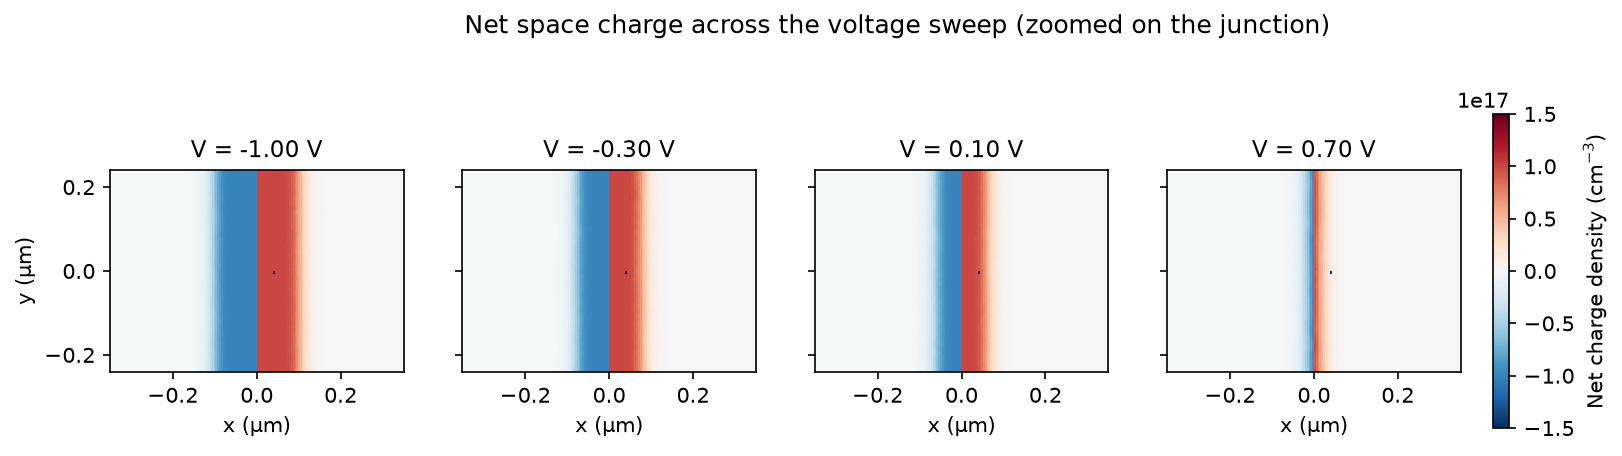
\includegraphics[width=\linewidth]{charge_animation_frames.png}
    \caption{Net space-charge density at four points in the voltage sweep, zoomed in on the junction. The depletion region (the colored band) visibly narrows going from reverse bias (left) to forward bias (right) -- the same behaviour shown as an interactive animation in the notebook version of this tutorial.}
    \end{figure}



    % Add a bibliography block to the postdoc
    
    
    
\end{document}
